\documentclass[conference]{IEEEtran}
\usepackage{graphicx}
\usepackage{amsmath}
\usepackage{booktabs}
\usepackage[caption=false]{subfig}
\graphicspath{{figures/}}
\begin{document}

\title{VOLLEY: A Linear-Motor Electromagnetic Deployment System for Deterministic CubeSat Orbit Seeding from Small Launch Vehicles}

\author{\IEEEauthorblockN{Adityavardhan Mishra}
\IEEEauthorblockA{Department of Mechanical Engineering, Symbiosis Institute of Technology\\
Symbiosis International (Deemed University), Pune, India\\
PRN 23070125054}}

\maketitle

\begin{abstract}
Secondary payloads on rideshare missions inherit the orbit of the primary customer, and the spring deployers that release them impart 1--2~m/s, too little to alter that orbit in any useful way. This paper presents the design and analysis of VOLLEY, a magazine-fed electromagnetic deployer that ejects unmodified CubeSats at a programmable velocity an order of magnitude above spring systems while remaining within standard qualification loads. On-orbit electromagnetic launch of CubeSats has been studied before, at velocities twenty times higher but at accelerations of order $10^3$~g and with a conductive armature attached to the payload \cite{feng2025}; the contribution claimed here is not electromagnetic deployment as such but the combination of a programmable velocity with a satellite that is never modified and an acceleration inside its existing qualification envelope. An architecture trade selects an ironless double-sided Halbach-array linear synchronous motor driving a reusable permanent-magnet sled along a 1.5~m track, with twelve 3U satellites fed from two transverse cassettes, a contactless eddy-current arrest brake, and supercapacitor pulse power. A winding-resolved motor model, cross-checked against an independent magnetostatic computation, gives a thrust constant of 11.2~N per kA/m with $\pm$1.3\% ripple and an exit velocity of 16.5~m/s for a 3U payload at 10.7~g, drawing 2.88~kJ per shot at 19\% electrical\-to\-payload efficiency (64\% total electrical-to-kinetic conversion, the sled's share being dissipated in the arrest brake by design). The velocity follows from a sled mass measured at 9.4~kg from the detailed CAD solids; an earlier parametric estimate of 4.9~kg gave 20.4~m/s, and the decision to adopt the measured value was fixed in advance of the structural analysis that tested it. Closed-loop simulation with realistic sensing yields a velocity dispersion of 0.027~m/s (3$\sigma$) about a 16.2~m/s fleet setpoint, equivalent to $\pm$0.10~km of apogee placement. One maximum-velocity ejection multiplies a propulsion-less satellite's orbital lifetime by 1.62; an independent propagator reproduces the multiplier at mean and high solar activity but not at low, so the ratio is quoted at a stated activity level and is not claimed invariant, and differential ejection velocities of 2--10~m/s establish 30$^\circ$ constellation spacing in 1.4--6.9 days against 25 days for differential-drag phasing under identical assumptions. A solid model closes the system at 77~kg dry and 125~kg loaded. Host integration is developed generically for any restartable upper stage or hosted platform, with ISRO's POEM and Skyroot's Vikram-1 kick stage analyzed as candidate first hosts.
\end{abstract}

\begin{IEEEkeywords}
CubeSat deployment, electromagnetic launch, Halbach array, linear synchronous motor, rideshare, constellation phasing, small launch vehicles.
\end{IEEEkeywords}

\section{Introduction}
The rideshare model has cut the cost of reaching orbit for small satellites, and it has done so by removing their choice of destination. A CubeSat manifested as a secondary payload is released wherever the primary customer's mission ends, through a spring deployer whose 1--2~m/s separation velocity exists for clearance rather than for orbit shaping. Satellites that carry propulsion can correct for this. The large class that cannot, which includes most university missions and cost-constrained commercial payloads, remains wherever it was dropped, at whatever altitude and phasing the manifest happened to produce.

Two families of hardware bracket the problem. Below it sit flight-proven springs, typified by the J-SSOD at 1.1--1.7~m/s \cite{jssod} and commercial deployers near 2~m/s \cite{exopod}. Above it sit propulsive orbital transfer vehicles, which move an entire bus through hundreds of m/s at a cost, mass, and integration burden far beyond what a 4~kg satellite needing a 20~m/s nudge can justify. Between the two lies a regime unserved \emph{by flown hardware}: no deployment system in service operates in the tens of m/s, although the astrodynamic utility of that band is substantial and quantifiable. The band is not unexamined in the literature. Feng \emph{et al.} simulate an on-orbit three-stage induction coilgun accelerating a 20~kg CubeSat to 321.56~m/s and map the resulting reachable domain \cite{feng2025}, and a sustained line of work from a second group develops magazine-fed electromagnetic transfer and release of stacked CubeSats, carried as far as a measured prototype of the transport mechanism \cite{stacked2022,xu2024,storage2025}. The contribution claimed here is therefore narrower and specific: a programmable exit velocity delivered to an \emph{unmodified} satellite within its own qualification envelope. Both qualifiers do work. An induction coilgun accelerates a conductive armature, which must either be attached to the customer satellite or separated as a sabot. And the velocity such a machine makes available is bounded in practice not by the machine but by the payload: Feng's 321.56~m/s is reached over a 3.9~m barrel, a mean acceleration of $1.35\times10^3$~g, with a reported peak force above 600~kN on a 20~kg body---some $3\times10^3$~g---against the 14~g quasi-static qualification level a standard CubeSat is built to \cite{gevs}. That gap, not the achievable speed, is what confines useful exit velocity to the tens of m/s, and it is the constraint this design was built around.

This paper develops a system for that band and keeps the treatment deliberately host-agnostic: the deployer is specified against a generic interface that any restartable upper stage, kick stage, or hosted orbital platform can satisfy, and specific vehicles enter only as worked candidate examples. The contributions are (1) an architecture trade showing why a linear synchronous motor rather than a coilgun is the correct electromagnetic topology at CubeSat structural limits; (2) a complete system design covering magazine, restraint, arrest, power, and abort; (3) a winding-resolved electromagnetic model, independently verified, together with ten quantitative analyses spanning launch performance, astrodynamics, deployment safety, and host interaction; and (4) a generalized integration framework with capacity and recoil budgets evaluated for candidate hosts in the Indian launch ecosystem.

\section{Related Work}
\subsection{Deployment heritage}
The P-POD established the rail-and-spring standard, and the ISS-based J-SSOD and NanoRacks systems industrialized it \cite{jssod,soa}. The failure record is instructive: the NanoRacks ball-lock anomaly, in which jack-screw preload above 0.11~N$\cdot$m drove the release mechanism toward seizure, traced to a load path in which ascent preload passed through the release device itself \cite{lewis}. VOLLEY's restraint architecture is designed against precisely this fault class. The closest electromagnetic relative is a proposed multi-CubeSat deployer using permanent-magnet conveying and ejection stages, demonstrated at 0.4--1.4~m/s \cite{mdpi}; VOLLEY extends the same Lorentz-force principle to roughly fifteen times that velocity.

\subsection{Electromagnetic launch and supporting technology}
Coilgun research examined nanosatellite launch at km/s scales \cite{turman,kaye}, establishing contactless acceleration and its costs: single-stage reluctance coilguns convert 1--2\% of stored energy into kinetic energy. Ironless permanent-magnet linear machines occupy the opposite corner of the design space: the Halbach array concentrates flux on one working face \cite{halbach}, and the Inductrack program demonstrated large forces from such arrays with no iron and no sliding contact \cite{inductrack}. Space-qualified supercapacitors have progressed to an established supply chain through ESA-led programmes \cite{faure,espc}. Eddy-current dampers carry decades of flight heritage in deployment mechanisms \cite{eddy}. On the astrodynamics side, Planet Labs demonstrated propulsion-free constellation phasing by differential drag over campaigns of weeks to months \cite{foster,foster2}; that timescale is the benchmark against which impulsive seeding is measured. ISRO's POEM programme converted the spent PSLV fourth stage into a stabilized hosted-payload platform across four missions, closing POEM-3 with a controlled, debris-free reentry \cite{poem3,poem4}, establishing the regulatory template for operating equipment on a spent stage.

\section{System Architecture}
\subsection{Requirements}
The driving requirements are: eject an unmodified 3U CubeSat, imposing no armature, plating, or electrical interface on the customer satellite; keep payload acceleration within standard qualification loads (25--30~g); fit an ESPA-Grande-class envelope and mass allocation, a requirement the current geometry does not yet meet (Sec.~\ref{sec:lim}); provide per-satellite programmable velocity with dispersion small against its astrodynamic effect; carry a twelve-satellite manifest with autonomous sequencing; provide inhibits and a defined abort; and hand recoil to the host in a form its attitude control absorbs at negligible propellant cost.

\subsection{Derivation of Principal Design Parameters}
The values that define the machine are set by requirements and standards rather than chosen freely; Table~\ref{tab:derive} records the governing relation for each. Three deserve explicit statement. The acceleration ceiling follows from the CubeSat Design Specification qualification environment: NASA GEVS \cite{gevs} protoflight random vibration integrates to 14.1~$g_{\mathrm{rms}}$, whose $3\sigma$ envelope of roughly 42~$g$ bounds the launch load, and a 25~$g$ design cap preserves margin against it. An earlier version of this design was acceleration-limited: at a 4.9~kg parametric sled the ejection ran at 16.3~$g$, close enough to the cap that the cap set the velocity through $v_{\max}=\sqrt{2a_{\max}L}$. That is no longer the binding constraint. With the sled measured at 9.4~kg the same commanded force accelerates a heavier moving mass, so the ejection sits at 10.7~$g$ and the 1.3~m zone yields 16.5~m/s. The machine is now \emph{thrust-and-mass} limited rather than acceleration-limited, with more than a factor of two of qualification margin left unused. Recovering velocity therefore means removing sled mass or raising sheet current, not shortening the stroke; a 0.2~m coast-trim zone completes the 1.5~m axis. Stroke buys velocity only as $\sqrt{L}$, so the trade is unattractive: total track lengths of 1.0, 1.2, 1.5 and 1.8~m give 13.0, 14.5, 16.5 and 18.3~m/s respectively, and the envelope is already the binding packaging constraint (Sec.~\ref{sec:lim}). The capacitor bank follows from the shot energy and the droop it actually reaches: at the 2.88~kJ draw the selected 6~F bank sags to $V_1=0.946V_0$, and
\begin{equation}
C=\frac{2E}{V_0^2-V_1^2}=5.99~\mathrm{F}\rightarrow 6~\mathrm{F},
\end{equation}
realized as thirty-two series 190~F, 3~V commercial cells for a 96~V rail compatible with 1200~V SiC devices at a comfortable derating.

\begin{table}[t]
\caption{Governing relation for each principal parameter}
\label{tab:derive}
\centering\footnotesize
\begin{tabular}{lll}
\toprule
Parameter & Value & Set by\\
\midrule
Accel. cap & 25 $g$ & GEVS 14.1 $g_{\mathrm{rms}}$, $3\sigma$ \cite{gevs}\\
Track length & 1.5 m & $v=\sqrt{2aL}$ + coast zone\\
Rail material & 7075-T6, hard anodize & CDS rail spec \cite{cds}\\
Bank voltage & 96 V & SiC 1200 V derated 60\%\\
Bank capacitance & 6 F & droop eqn (2), $\le$5\% SoC sag\\
Sled magnets & N45SH & thermal $\times$ field (Sec.~V-F)\\
Brake cap & 200 $g$ sled & magnet bond MoS (Sec.~III-F)\\
Abort point & 45\% stroke & braking-distance equality\\
Magazine & 12 (2$\times$6) & cassette CoM symmetry\\
\bottomrule
\end{tabular}
\end{table}

\subsection{Topology Trade}
The payload settles the trade before the electromagnetics do. Exit velocity is bounded by
\begin{equation}
v_{\max}=\sqrt{2\,a_{\max}L},
\end{equation}
so at 25--30~g over a 1.3--2~m stroke the ceiling is 26--35~m/s. The coilgun's defining advantage, a km/s-class ceiling, is unreachable by the payload it would carry, while its costs remain: 1--2\% single-stage efficiency \cite{turman}, microsecond timing against the suck-back effect, and an armature bolted to the customer's satellite. A linear synchronous motor concedes nothing in the reachable envelope and inverts every cost: high drive efficiency, continuous servo control, and a reusable sled that carries the magnets so the satellite carries nothing. Table~\ref{tab:trade} summarizes.

\begin{table}[t]
\caption{Topology trade at CubeSat structural limits}
\label{tab:trade}
\centering\footnotesize
\begin{tabular}{lcc}
\toprule
Criterion & Reluctance coilgun & Ironless LSM + sled\\
\midrule
Velocity ceiling (payload-limited) & 26--35 m/s & 26--35 m/s\\
Electrical$\rightarrow$payload efficiency & 1--2\% \cite{turman} & 19\% (Sec.~V)\\
Satellite modification & armature required & none\\
Velocity control & pulse timing & closed-loop servo\\
Abort & none once fired & to $\sim$45\% stroke\\
Field on stored satellites & pulsed, unshielded & Halbach self-shielded\\
\bottomrule
\end{tabular}
\end{table}

\subsection{Layout and Firing Cycle}
The launcher is organized around a single 1.5~m track: a 1.3~m acceleration zone and a 0.2~m coast-and-trim zone (Figs.~\ref{fig:block} and \ref{fig:layout}). The stator is an ironless double-sided three-phase copper winding; the mover is a 4.9~kg sled carrying opposed Halbach arrays (48~mm wavelength, 8~mm N45SH blocks, four blocks per wavelength) across a 12~mm winding gap. Two transverse cassettes of six 3U satellites flank the breech. The cycle: a follower advances one pitch and slides a satellite laterally onto the sled cradle (a sub-newton operation in microgravity); a detent latch engages; a two-finger escapement retains the next satellite; the motor accelerates the stack; force is removed in the coast-trim zone where the servo makes its final correction; the sled enters the brake and decelerates while the satellite departs along guide extensions. Retention during acceleration costs nothing, since inertia presses the satellite into the aft backstop, and release costs nothing, since braking the sled is the release. Cadence is set by supercapacitor recharge, 10--20~s at a 150--300~W allocation.

\begin{figure}[t]
\centering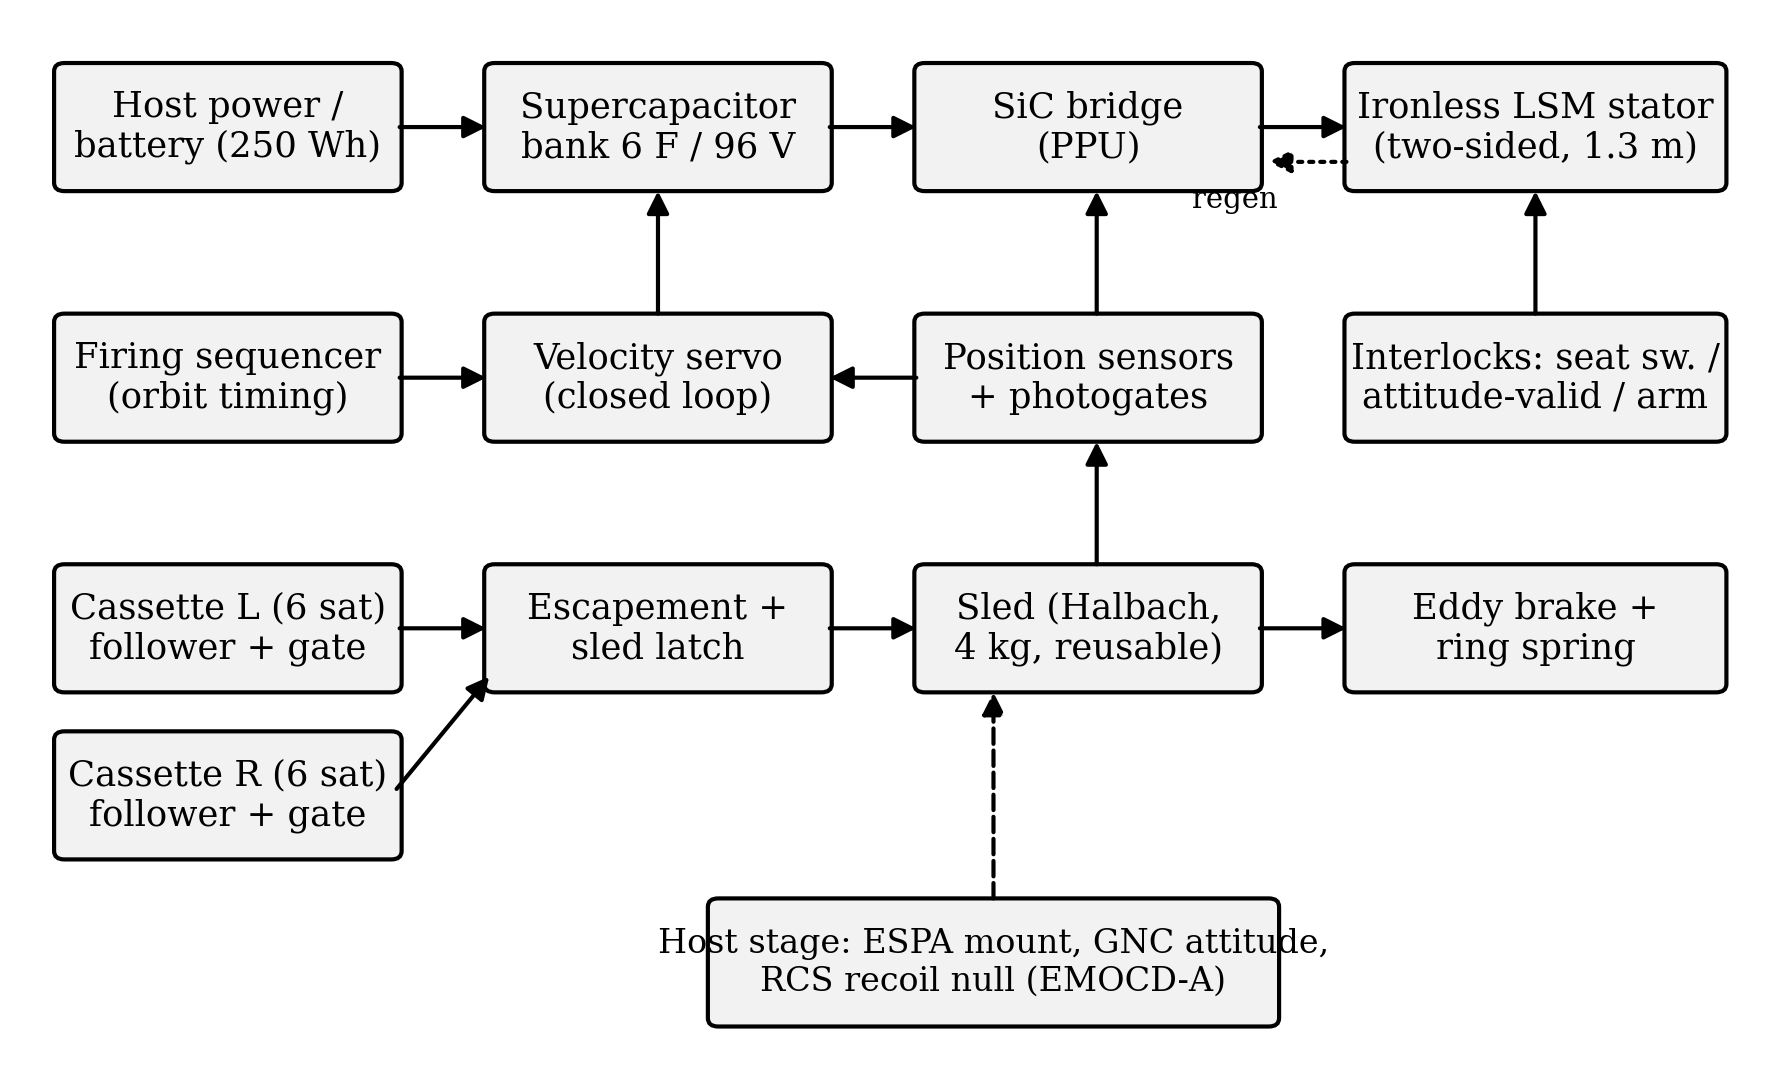
\includegraphics[width=\columnwidth]{D01_block.png}
\caption{System block diagram: power, control, mechanism, and host-interface chains.}
\label{fig:block}
\end{figure}

\begin{figure}[t]
\centering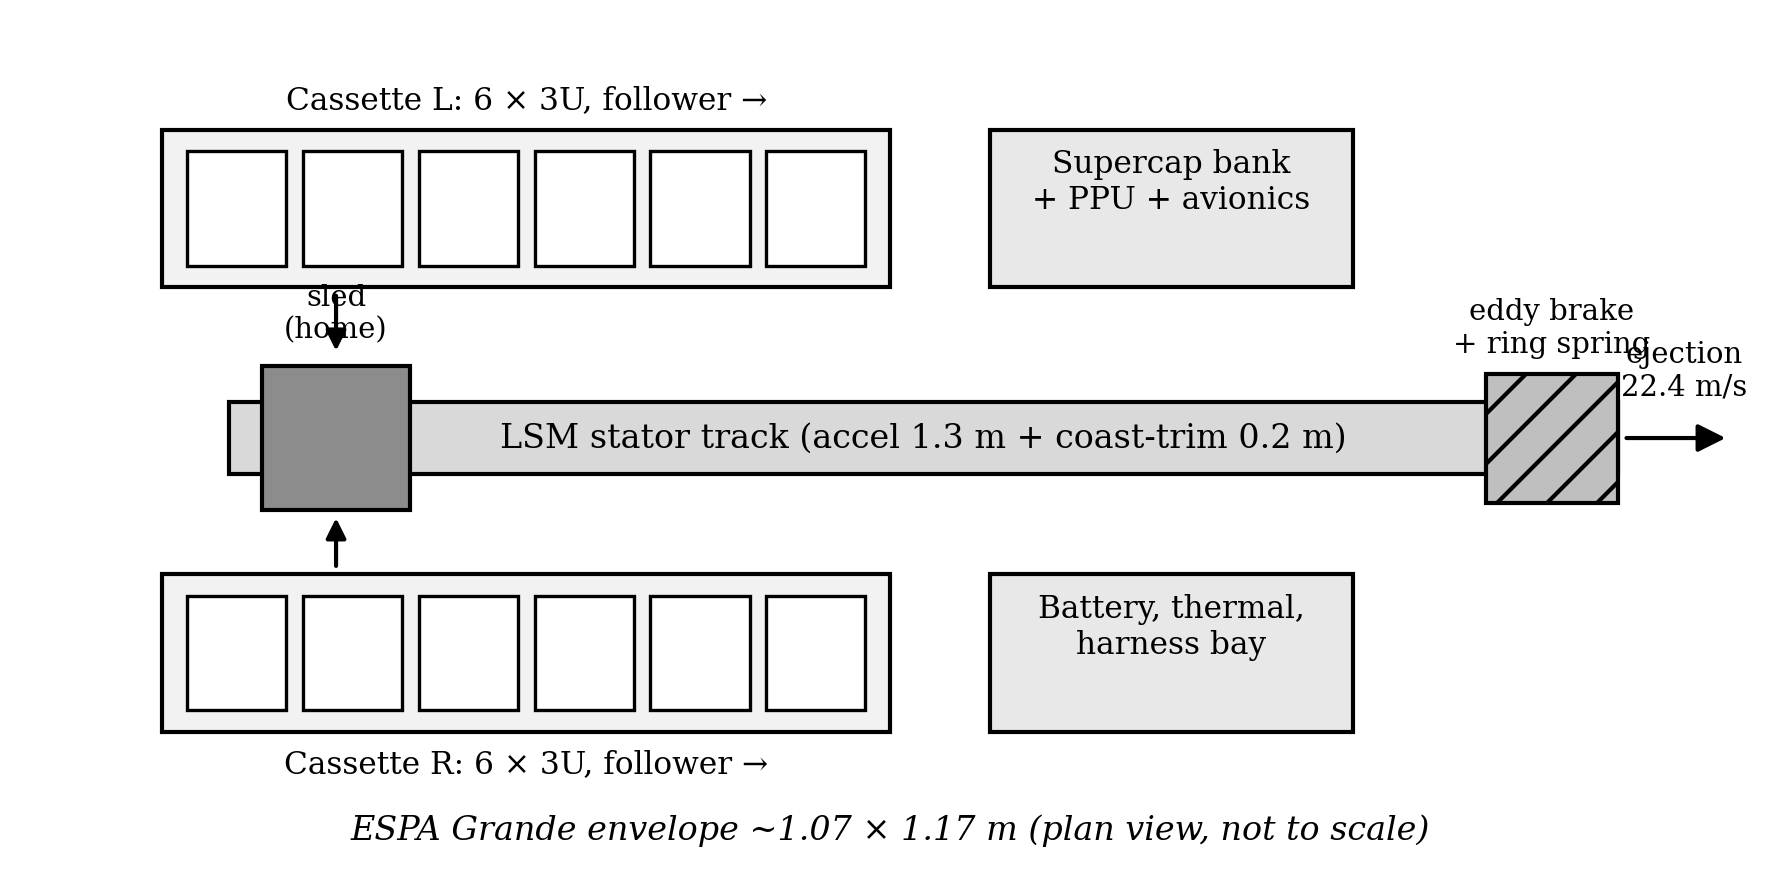
\includegraphics[width=\columnwidth]{D02_layout.png}
\caption{Plan-view layout against an ESPA-Grande-class envelope (not to scale). The closed envelope currently exceeds that class in length; see Sec.~\ref{sec:lim}.}
\label{fig:layout}
\end{figure}

\subsection{Restraint, Inhibits, and Abort}
Launch restraint separates the preload path from the release path, the inverse of the NanoRacks fault \cite{lewis}. One-shot retention gates at each cassette exit carry ascent preload directly into structure; the escapement is caged during ascent; the sled is held by a motorized over-center cam lock. Firing requires a three-inhibit chain: redundant seat switches, an attitude-valid flag from the host, and a sequencer arm. Abort is available to approximately 45\% of the stroke, beyond which braking distance for the combined mass exceeds remaining track; the muzzle buffer is sized to capture an aborted combined mass. The retention gate carries the ascent preload of a six-satellite stack, $24\,\mathrm{kg}\times25\,g=5.9$~kN, through two D6 A-286 shear pins (double-shear capacity 18.2~kN, margin 1.2 on ultimate at a 1.4 design factor); the escapement, caged behind the gate, sees none of this. The abort threshold is where the sled braking distance under the same thrust equals the remaining track, which for the loaded 13.4~kg carriage falls at 45\% of stroke and 11.1~m/s. The commit fraction is unchanged by the heavier sled---braking distance and travelled distance scale with mass identically, so the mass cancels---but the velocity at the commit point falls with the acceleration.

\subsection{Arrest, Power, and Materials}
The sled arrives at the brake with about 1.29~kJ. Motor regeneration alone cannot arrest it, because braking force is bounded by the same thrust constant as acceleration. A copper-fin eddy-current brake provides bulk arrest: force proportional to velocity, contactless, with flight heritage in the damper class \cite{eddy}. Authority is abundant, so the pole entry is tapered to cap sled deceleration near 200~$g$. This limit is set by the magnet retention: a 65~g Halbach block at 200~$g$ loads its bonded interface (10.8~cm$^2$) to only 0.12~MPa against a conservative 10~MPa epoxy allowable, a margin of 84, so 200~$g$ is a deliberate conservatism protecting the brittle sinter rather than a strength limit. The 0.86~kg copper fin absorbs the sled's 1.29~kJ per shot at an adiabatic 3.9~K per-shot transient rise, radiating between shots; a ring-spring catches the residual below 1.5~m/s (Fig.~\ref{fig:brake}). Pulse energy comes from a 6~F, 96~V supercapacitor bank switched by a SiC bridge \cite{faure}. Materials follow three rules: nothing conductive rides the changing field (titanium sled chassis, PEEK formers), nothing near the track is ferromagnetic except by design (BeCu springs, A-286 fasteners), and nothing outgasses near customer optics (E595-compliant polymers, dry films, sealed roller cartridges).

\begin{figure}[t]
\centering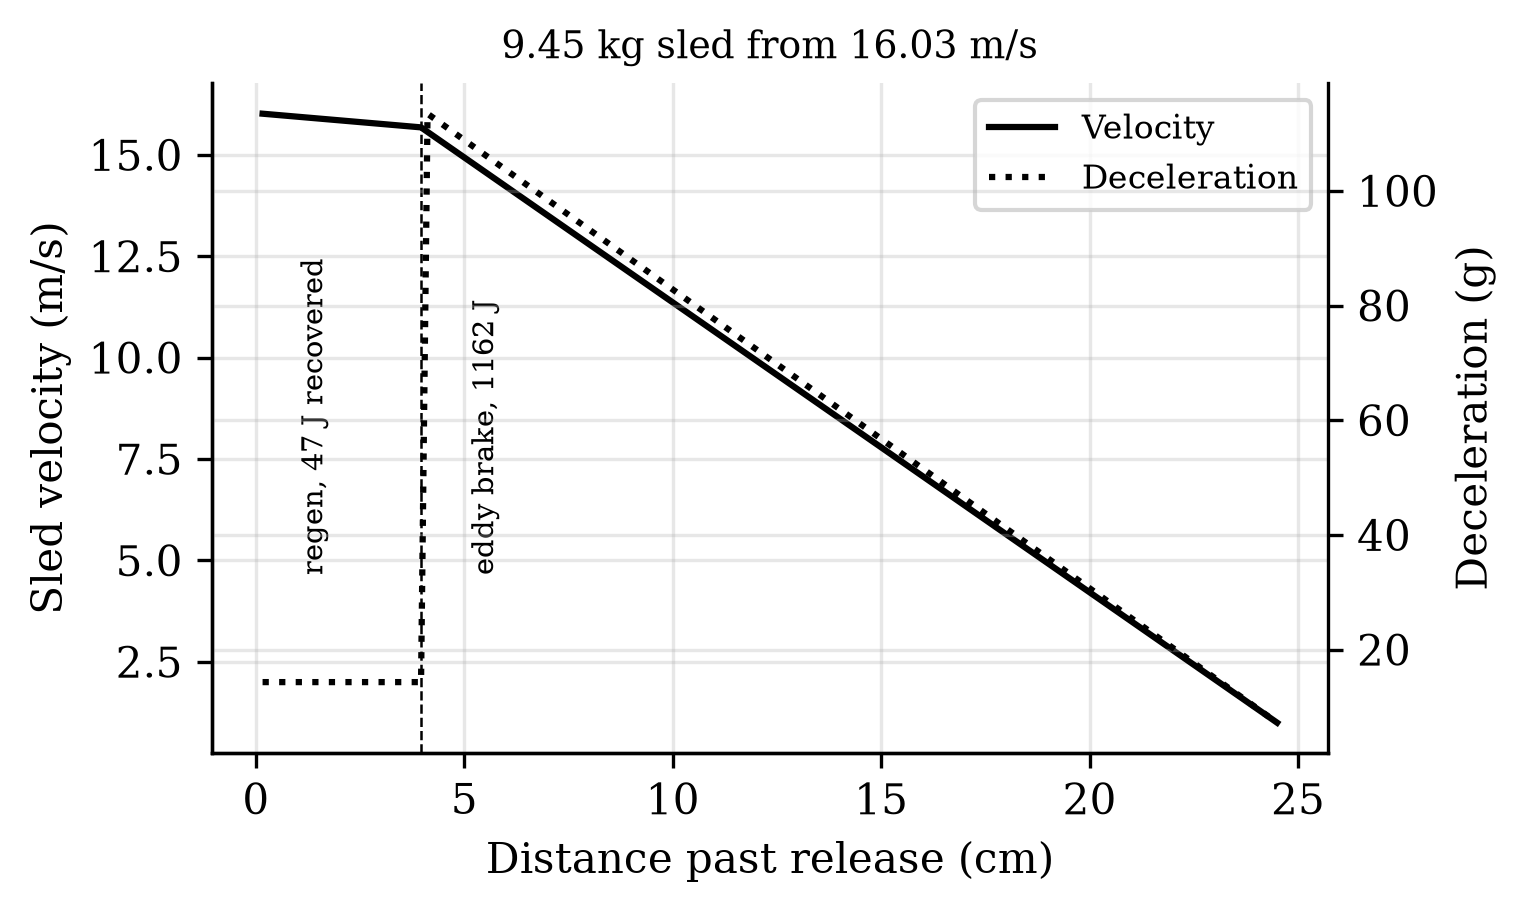
\includegraphics[width=0.85\columnwidth]{F08_brake.png}
\caption{Eddy-brake arrest, taper-limited to 200~g on the sled.}
\label{fig:brake}
\end{figure}

\section{Models and Verification}
\subsection{Field Model and Independent Verification}
The Halbach airgap field is a decaying wave, $B(y)=B_0e^{-ky}$ with $k=2\pi/\lambda$, summed over the two opposed faces. Because this carries the force budget, it was checked against an independent magnetostatic computation (analytic cuboid superposition, magpylib), with the array rotation-sense convention determined empirically by probing a single array on both faces; the exercise caught two successive sign errors whose outputs matched single-array fingerprints. Converged results: single-array mid-gap 0.351~T against the wave model's 0.351~T; double-sided mid-gap peak 0.694~T against a predicted 0.702~T. The stray field behind the array back face, which sets the magnetic keep-out for stored satellites, computes to 22.7~mT at 10~mm, 4.3~mT at 20~mm, and 0.4~mT at 50~mm.

\subsection{Winding-Resolved Thrust Constant}
A slotless three-phase belt winding (pole pitch $\lambda/2$, belts of $\lambda/6$, winding factor 0.955) was resolved against the verified field by direct Lorentz integration with position-locked sinusoidal commutation, the field translated with the sled. The result is a thrust constant
\begin{equation}
K_t = 11.22~\mathrm{N\,per\,kA/m},\qquad \text{ripple } \pm1.26\%\ (6\text{th harmonic}),
\end{equation}
shown in Fig.~\ref{fig:ripple}. Synchronous extraction carries the one-half traveling-wave factor that lumped $\langle B\rangle KA$ models hide; the corrected constant is recovered operationally by rating the sheet current at 140~kA/m and commanding 126~kA/m (21~A/mm$^2$ pulse-only in the copper), where adiabatic heating remains 0.3~K per 157~ms shot.

\begin{figure}[t]
\centering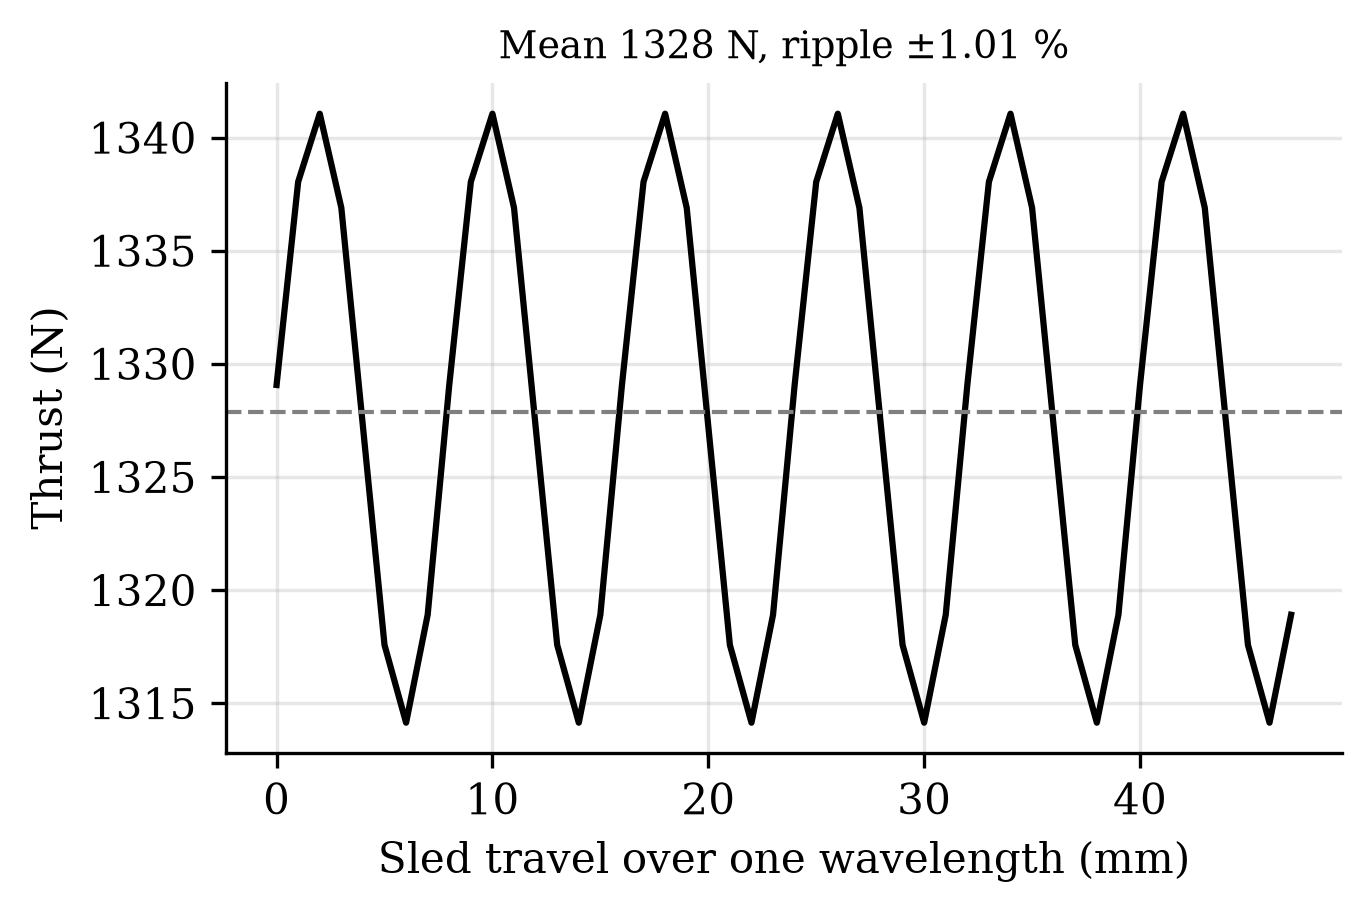
\includegraphics[width=0.8\columnwidth]{F02_ripple.png}
\caption{Winding-resolved thrust over one wavelength of sled travel.}
\label{fig:ripple}
\end{figure}

\subsection{Shot, Servo, and Astrodynamic Models}
The shot integrates sled-plus-satellite dynamics against the supercapacitor circuit with explicit copper loss and a 95\% converter. Velocity control uses a position-scheduled profile with proportional correction and a coast-trim residual correction from photogate measurement; an 800-run Monte Carlo over thrust-constant, mass, force-ripple, and sensor tolerances gives the dispersion. Orbital lifetime uses per-revolution orbit-averaged decay (Gauss tangential equations, quadrature over eccentric anomaly, static exponential atmosphere at mean activity \cite{vallado}); the method was cross-validated against an independent Cowell RK4 propagation with drag, the two agreeing on 30-day semi-major-axis decay to 99.4\%. Constellation seeding uses $\Delta a = 2a\,\Delta v/v$ and the resulting period difference; deployment safety propagates the stage and all deployed ellipses with Kepler-plus-secular-$J_2$ motion for 30 days, with candidate minima refined at 0.25~s sampling.

\section{Performance Results}
\subsection{Launch Performance}
At the rated point (3U reference, 9.445~kg sled measured from the CAD solids, 1.3~m acceleration): exit velocity \textbf{16.5~m/s} at \textbf{10.7~g}, pulse 157~ms, peak current 347~A, bank state\-of\-charge sag 5.4\%, with roughly 4\% additional resistive dip at peak current (Fig.~\ref{fig:shot}). Energy drawn is 2.88~kJ per shot, with copper heat of 828~J and a further 86~J dissipated in the bank's own series resistance. The payload receives 547~J, a \textbf{19\% electrical\-to\-payload efficiency}; 64\% of drawn energy becomes kinetic energy overall, the sled's 1.29~kJ share being dissipated in the arrest brake by design rather than recovered. Efficiency falls with the heavier sled for two compounding reasons: a larger fraction of the same mechanical work goes into a mass that is then braked away, and the longer 157~ms pulse accrues more copper loss at unchanged current density. The closed-loop Monte Carlo returns a dispersion of \textbf{0.027~m/s (3$\sigma$)} at a 16.2~m/s fleet setpoint (Fig.~\ref{fig:mc}), dominated by the sensing chain rather than plant tolerances. The setpoint must sit below the open-loop ceiling for the servo to retain authority; at 98.2\% of it, the headroom is the same fraction the superseded 20.0~m/s setpoint held. Table~\ref{tab:family} gives the payload family: the system is force-limited above 1U, so heavier payloads trade velocity, never structural margin.

\begin{figure}[t]
\centering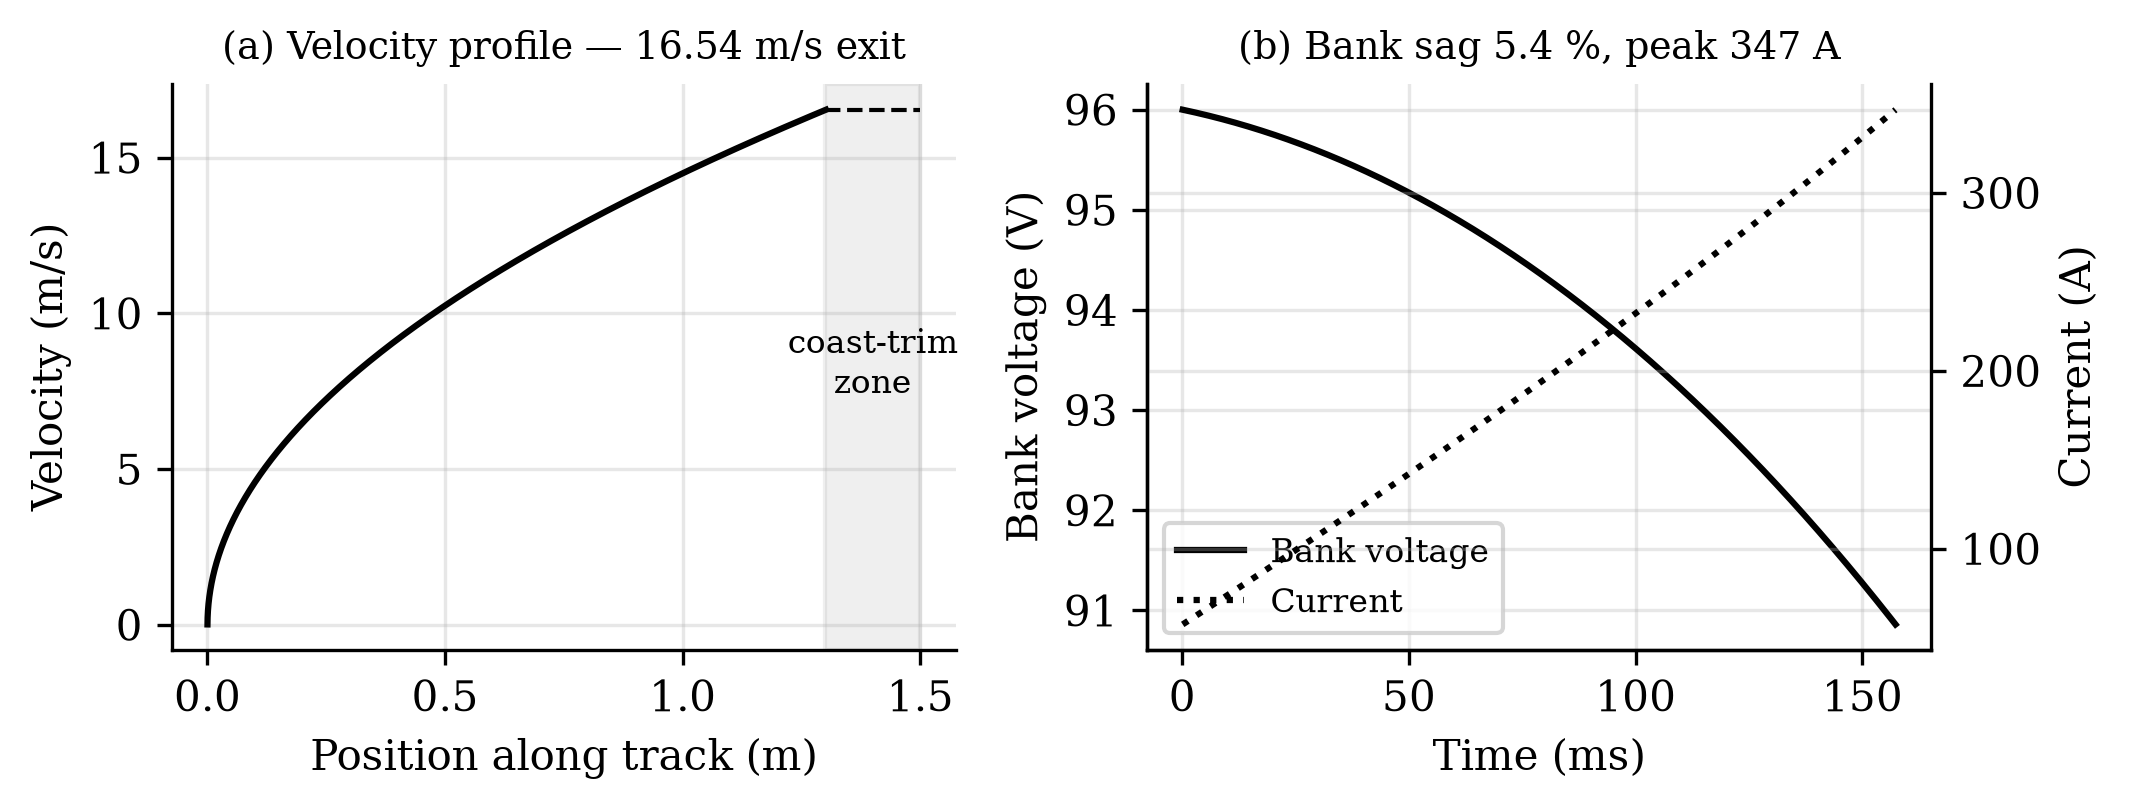
\includegraphics[width=\columnwidth]{F01_shot.png}
\caption{Shot profile at the rated point: (a) velocity with coast-trim zone; (b) bank voltage and current.}
\label{fig:shot}
\end{figure}

\begin{figure}[t]
\centering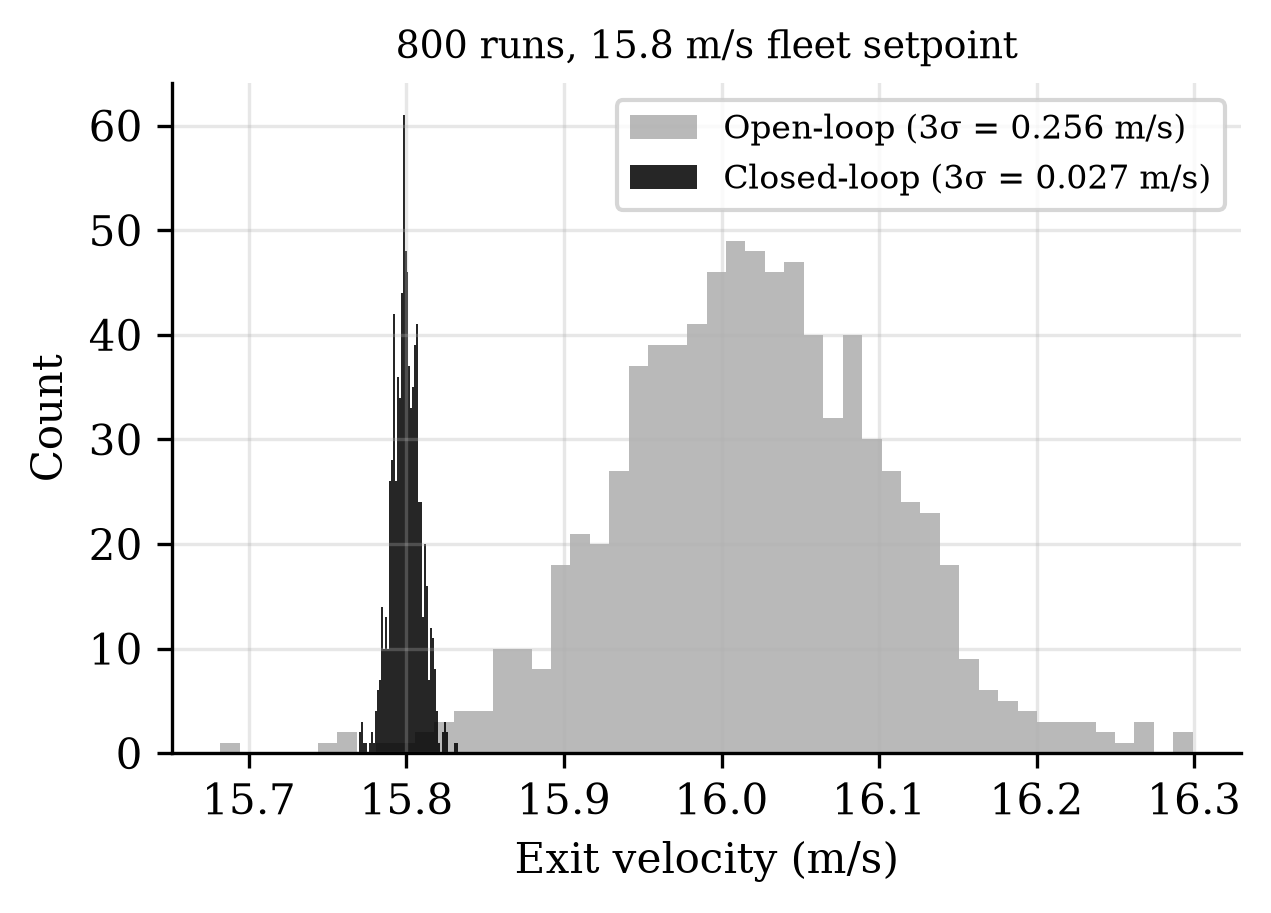
\includegraphics[width=0.8\columnwidth]{F03_mc.png}
\caption{Closed-loop exit-velocity dispersion, 800 Monte Carlo runs.}
\label{fig:mc}
\end{figure}

\begin{table}[t]
\caption{Payload family at the rated point (1.3 m acceleration, 9.445 kg measured sled)}
\label{tab:family}
\centering\footnotesize
\begin{tabular}{lcc}
\toprule
Class & Exit velocity & Acceleration\\
\midrule
1U (1.3 kg) & 18.5 m/s & 13.4 g\\
3U (4 kg) & 16.5 m/s & 10.7 g\\
6U (8 kg) & 14.5 m/s & 8.3 g\\
12U (12 kg) & 13.1 m/s & 6.7 g\\
\bottomrule
\end{tabular}
\end{table}

\subsection{Astrodynamic Utility}
A prograde ejection raises apogee while leaving perigee at the deployment altitude, so the correct claim is a longer-lived ellipse. At 450~km with ballistic coefficient 61~kg/m$^2$, one 16.5~m/s shot multiplies lifetime by \textbf{1.62} at mean solar activity (base lifetimes 0.52--2.61~yr across the activity range; Figs.~\ref{fig:life} and \ref{fig:uq}).

An earlier version of this work claimed the multiplier was invariant to two decimal places across ballistic coefficients of 40--90~kg/m$^2$ and across a fivefold density range, and offered that invariance as the result the analysis could defend. That claim does not survive an independent propagator. Run headless against MSISE90 with 20$\times$20 gravity, lunisolar third bodies and solar radiation pressure, GMAT R2022a reproduces the multiplier at mean and high activity but returns 2.07 at low activity, a spread of 18\% against a 5\% acceptance band fixed before the run. The reason is a defect in how the sweep was posed rather than in the arithmetic: the model represents solar activity as a uniform multiplicative scale on density, and ballistic coefficient enters the drag term in the same multiplicative slot, so both sweeps divide the two lifetimes being compared by the same factor. Their ratio cannot move, whatever the atmosphere does. A real atmosphere changes the \emph{shape} of the density--altitude profile with activity, the boosted orbit's apogee samples that profile some 37~km higher than the baseline's, and the ratio then does move. The multiplier is therefore quoted here at a stated activity level, and no invariance is claimed.

Differential ejection velocities put adjacent satellites on different periods: splits of 2, 5, and 10~m/s reach 30$^\circ$ spacing in \textbf{6.9, 2.8, and 1.4 days}. Under identical density and geometry assumptions, differential drag between 3:1 area configurations achieves the same spacing in \textbf{25.0 days} (Fig.~\ref{fig:dragvs}), consistent with flown drag-phasing campaigns operating over weeks to months \cite{foster}. Impulsive seeding followed by drag trim follows naturally as a hybrid.

\begin{figure}[t]
\centering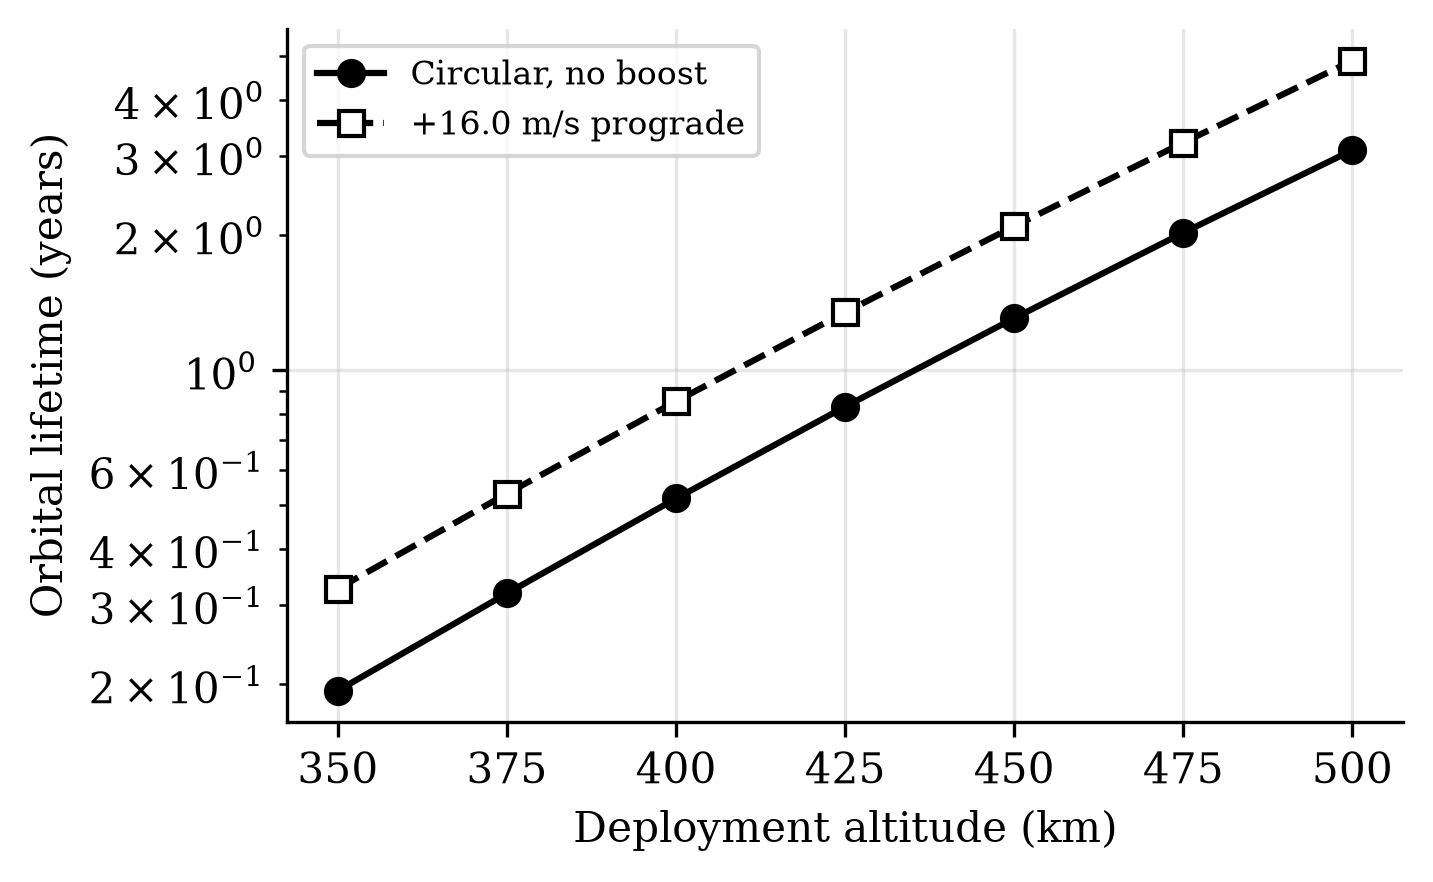
\includegraphics[width=0.85\columnwidth]{F04_life.png}
\caption{Orbital lifetime vs deployment altitude (BC = 61 kg/m$^2$, mean activity).}
\label{fig:life}
\end{figure}

\begin{figure}[t]
\centering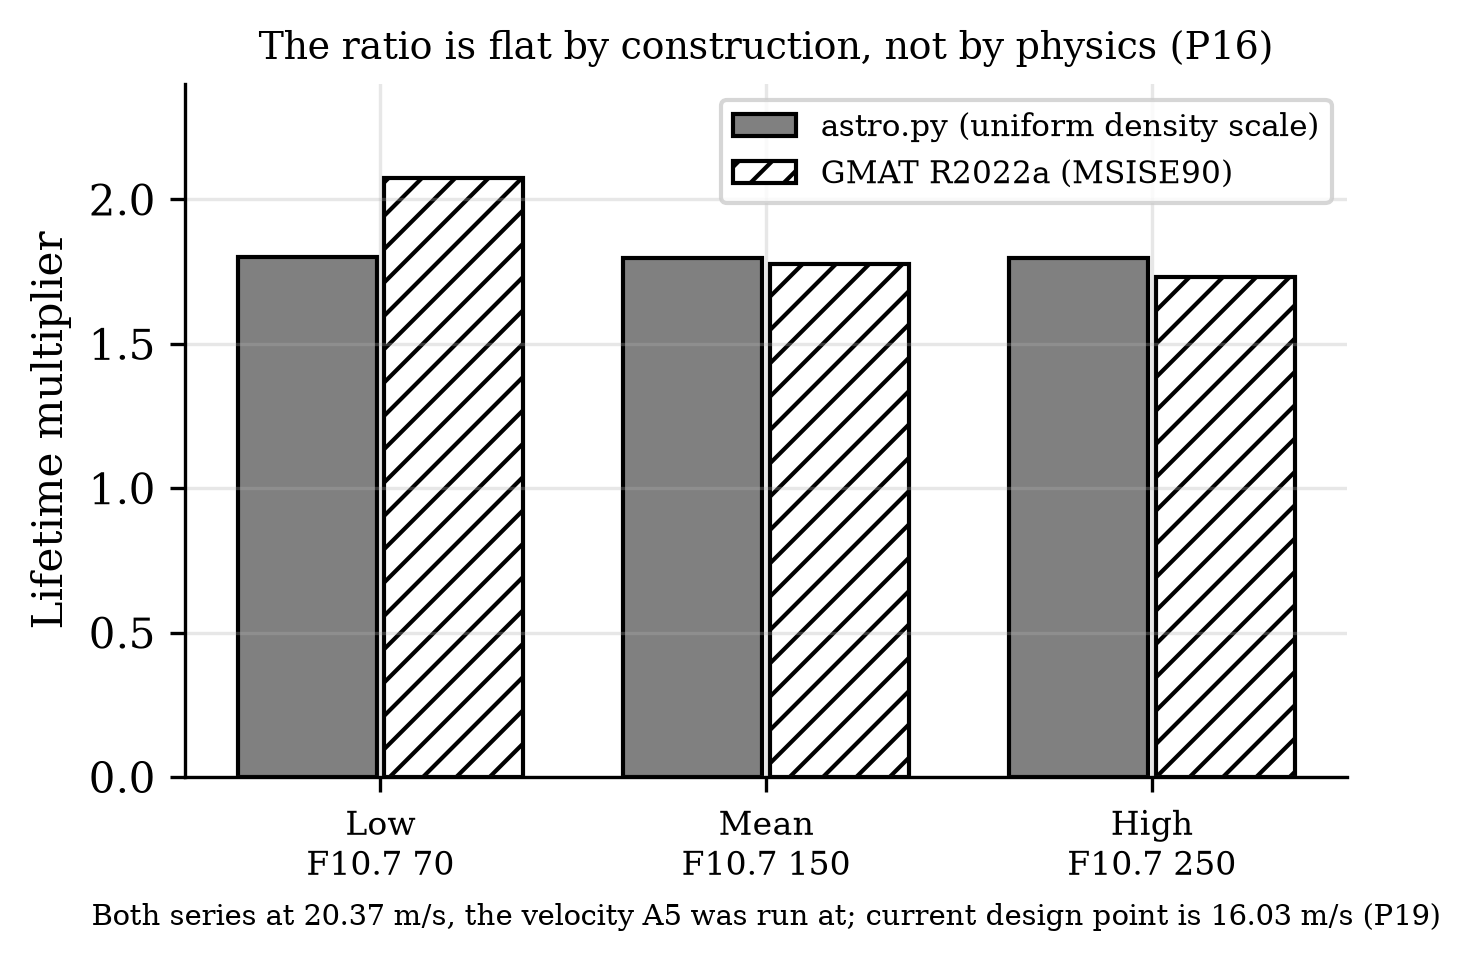
\includegraphics[width=0.8\columnwidth]{F11_uq.png}
\caption{Solar-activity sweep against GMAT. The static-atmosphere model returns a flat ratio by construction, not by physics; an independent propagator does not.}
\label{fig:uq}
\end{figure}

\begin{figure}[t]
\centering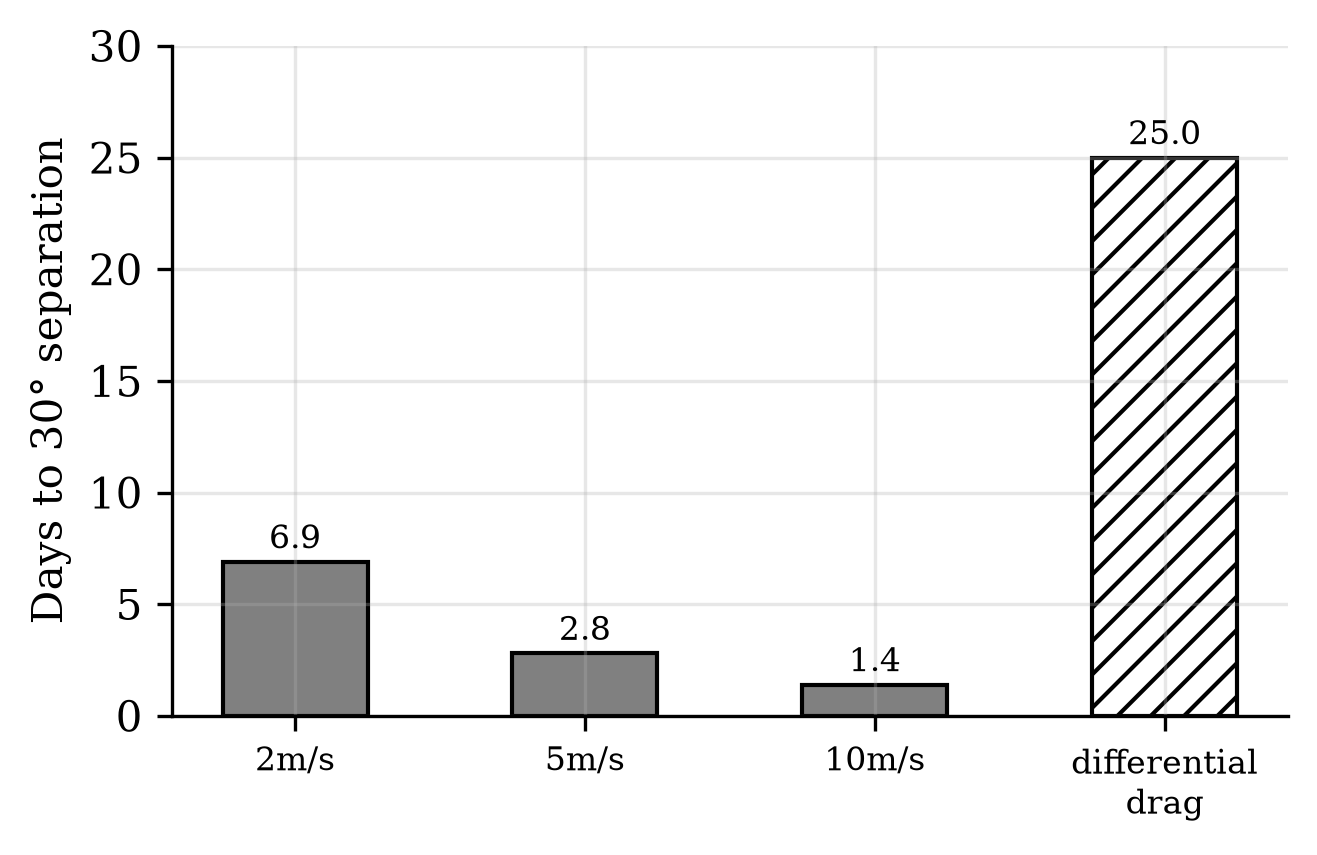
\includegraphics[width=0.85\columnwidth]{F05_dragvs.png}
\caption{Constellation seeding: VOLLEY velocity splits versus differential drag under identical assumptions.}
\label{fig:dragvs}
\end{figure}

\subsection{Deployment Safety}
Every prograde shot leaves an ellipse whose perigee sits at the firing altitude, so the fleet re-crosses the stage's orbit by construction, and the along-track phase between a deployed satellite and the stage realigns on a period of \textbf{9.9 days} at the rated velocity (Fig.~\ref{fig:conj}). The closest approach reached within a 30-day screening window is deliberately \emph{not} quoted here as a safety figure: because both bodies re-cross the same altitude, that minimum is fixed by the exact along-track phase at crossing, which is acutely sensitive to ejection velocity---in the model a $\pm2.5\%$ change about the rated point sweeps the 30-day minimum by more than an order of magnitude. It is a near-resonant sample of the beat geometry, not a design property. Two statements survive that sensitivity and carry the safety argument. First, per-shot collision-avoidance (COLA) screening is \textbf{mandatory} for every ejection, because the approach geometry cannot be certified from the nominal velocity alone. Second, disposing of the host stage before the first \mbox{9.9-day} realignment---routine for a restartable stage---removes the recurring close-approach mechanism at its source, before the fleet can return to the stage's along-track position. Per-shot conjunction products remain a mission-operations deliverable.

\begin{figure}[t]
\centering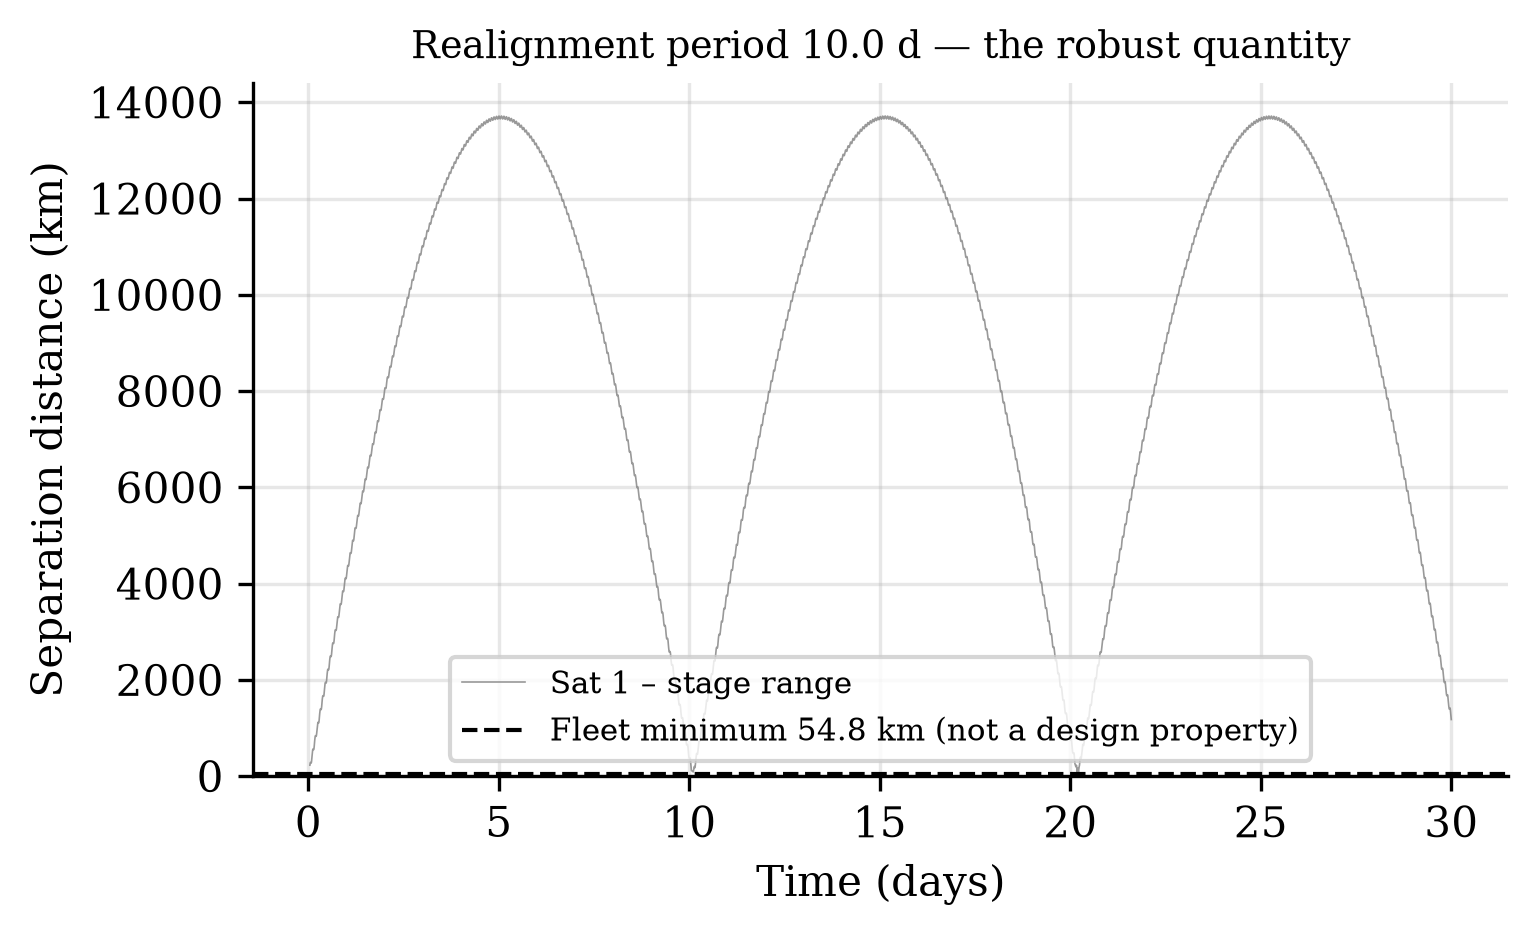
\includegraphics[width=0.85\columnwidth]{F06_conj.png}
\caption{Satellite--stage range over 30 days, staggered firing at the rated velocity.}
\label{fig:conj}
\end{figure}

\subsection{Error, Tip-Off, and Mass}
The 0.027~m/s dispersion maps to \textbf{$\pm$0.10~km apogee placement} at 450~km: sub-kilometre deterministic insertion for a satellite with no propulsion. The tip-off budget sums to 3.9~deg/s worst case against the 5~deg/s requirement class of ISS-heritage deployers \cite{nrcsd} (Fig.~\ref{fig:tipoff}); the coast-trim release is what closes it, since at full force the leading term alone would approach 34~deg/s. Recoil per shot is the satellite's momentum only, \textbf{66.1~N$\cdot$s}, the sled's share returning through the brake. The solid model closes dry mass at \textbf{76.9~kg} (loaded 124.9~kg, centre of gravity 0.44~m from the breech), with the ironless stator at 7.3~kg of copper and formers; the system uses roughly a third of an ESPA Grande \emph{mass} allocation. It does not currently fit the corresponding envelope: the closed CAD assembly measures 1839~mm along the track against the roughly 1270~mm of that class, because the arrest brake sits beyond the release point and the enclosure must span it. Resolving this means shortening the track, repackaging the brake, or accommodating on a host that does not impose the ESPA-Grande envelope; it is an open packaging item, not a solved one.

\begin{figure}[t]
\centering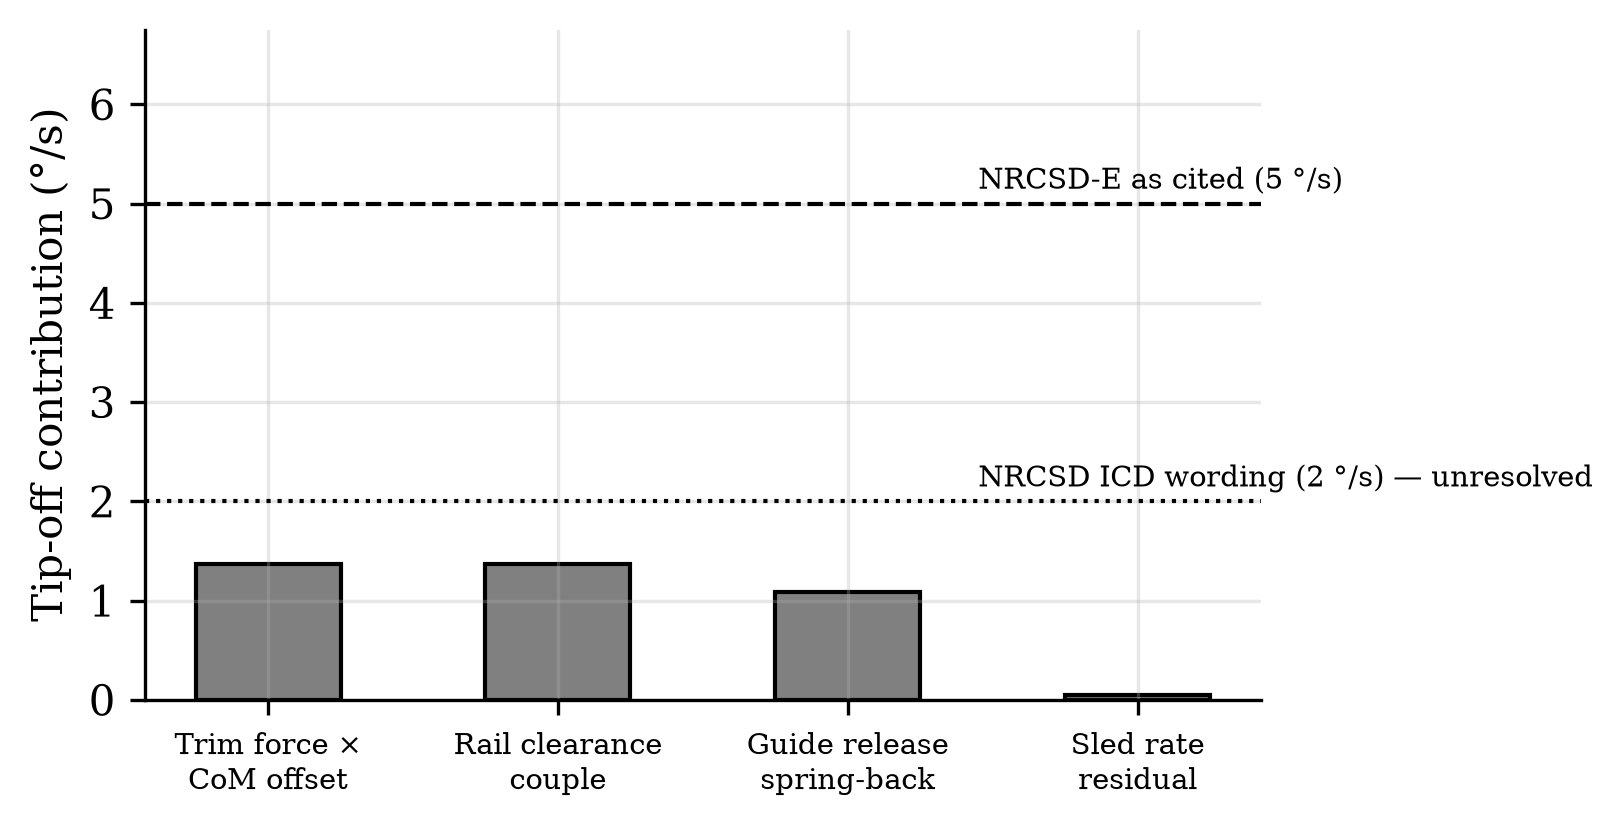
\includegraphics[width=0.8\columnwidth]{F09_tipoff.png}
\caption{Tip-off error budget against deployer requirement classes.}
\label{fig:tipoff}
\end{figure}

\begin{figure}[t]
\centering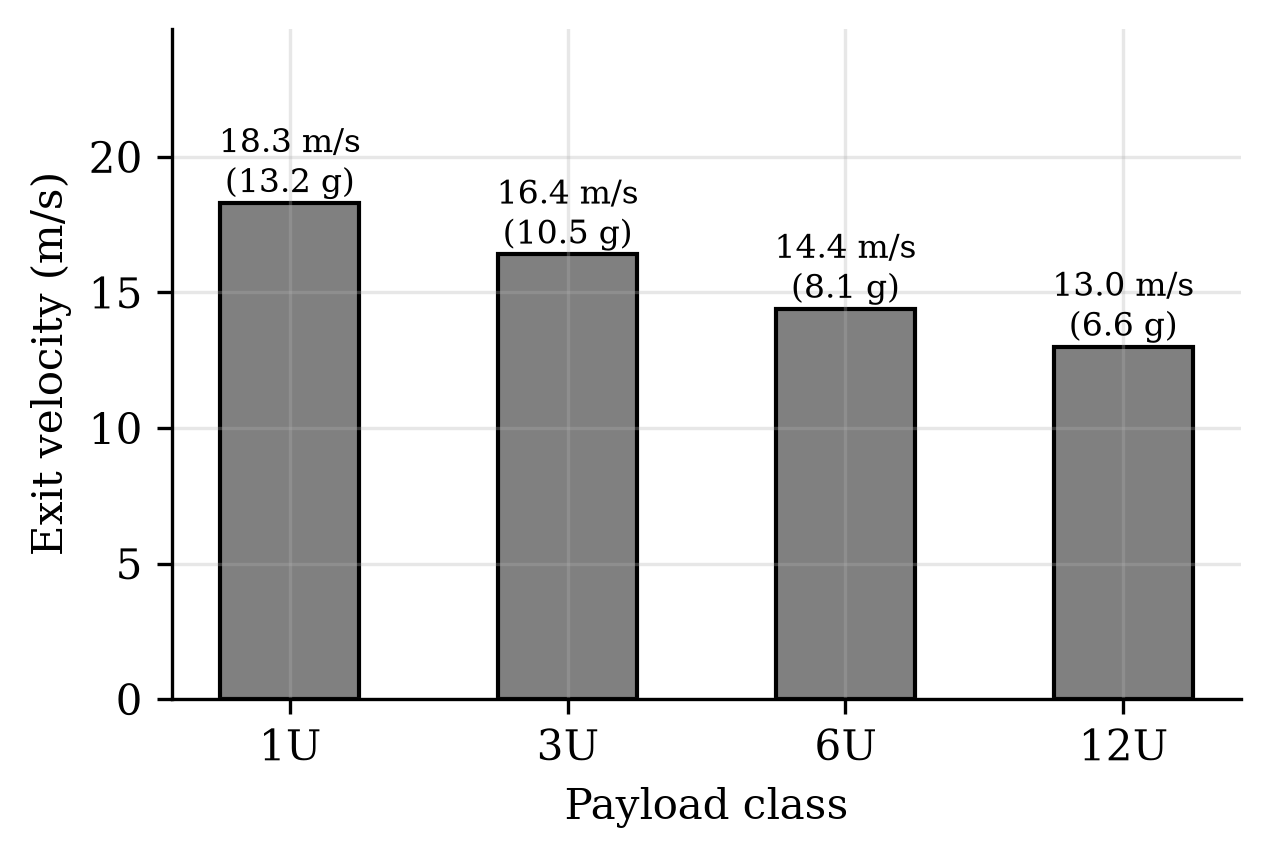
\includegraphics[width=0.8\columnwidth]{F07_family.png}
\caption{Payload family: force-limited above 1U; velocity, not safety, is traded.}
\label{fig:family}
\end{figure}

\section{Generalized Host Integration}
\subsection{Interface Requirements for Any Host}
VOLLEY-A, the attached mode analyzed here, requires four things of a host: a secondary-payload-class mechanical mount; 150--300~W of recharge power or an equivalent battery allocation; an attitude reference and enough control authority to null per-shot torque; and a disposal path consistent with debris rules. Nothing in the design binds it to one vehicle. Two recoil facts generalize across hosts. First, correction propellant depends only on total ejected momentum, about 0.98~kN$\cdot$s for a full manifest, roughly half a kilogram of hydrazine-class propellant regardless of host mass; host mass sets the per-shot rate disturbance, not the fuel bill. Second, the per-shot translation scales inversely with host mass (Table~\ref{tab:recoil}) and, for restartable stages, folds into disposal targeting. VOLLEY-F, a free-flyer variant with its own GNC, is the growth path for multi-day firing geometry and is not analyzed further here.

\begin{table}[t]
\caption{Per-shot recoil (66.1 N$\cdot$s) versus host class}
\label{tab:recoil}
\centering\footnotesize
\begin{tabular}{lcc}
\toprule
Host class & $\Delta V$ per shot & 12-shot total\\
\midrule
200 kg free-flyer & 408 mm/s & 4.9 m/s\\
300 kg kick stage & 272 mm/s & 3.3 m/s\\
600 kg kick stage & 136 mm/s & 1.6 m/s\\
900 kg (PS4 class) & 91 mm/s & 1.1 m/s\\
420 t (station class) & 0.2 mm/s & 2.3 mm/s\\
\bottomrule
\end{tabular}
\end{table}

\subsection{Candidate Hosts}
Any restartable kick stage, extended-mission upper stage, or hosted orbital platform satisfies the interface. Two Indian candidates are worked as examples because both exist today. ISRO's POEM is the flown precedent: a spent PS4 operated as a three-axis-stabilized hosted platform with solar power, NavIC navigation, and helium attitude thrusters, retired by controlled reentry \cite{poem3,poem4}; it supplies everything VOLLEY-A borrows, and its zero-debris closeout is the regulatory template. Skyroot Aerospace's Vikram-1 carries a restartable liquid Orbit Adjustment Module (one Raman-2 engine, four Raman Mini thrusters, eight cold-gas thrusters, stage-tested through more than a thousand pulses \cite{oam}) whose stated multi-orbit deployment role is functionally the PS4's; against the vehicle's published 350~kg LEO capacity \cite{spacenews}, a loaded VOLLEY is 34\%, falling to 22\% and 13\% on the announced 550~kg and 900~kg family members, so early flights are dedicated demonstrations and later ones ordinary manifest items. One integration quantity cannot be closed from public data: the OAM's mass and control authority are undisclosed \cite{oam}, which is why Table~\ref{tab:recoil} is parametric; obtaining stage mass, thruster impulse budget, and coast duration is the single data exchange that converts the analysis from parametric to specific for any candidate vehicle, Indian or otherwise. Comparable hosts elsewhere include kick stages evolved into mission platforms and ESPA-hosted propulsive rings; the interface asks the same four questions of each.

\subsection{Integration Interfaces}
The four-item interface resolves into concrete provisions. Mechanically the deployer bolts to a standard ESPA or ESPA-Grande ring through a canted bracket that passes the thrust line near the host centre of mass; the interface control document fixes the bolt pattern, envelope, and the published magnetic keep-out radius. Electrically it draws a 150--300~W recharge feed and a switched safety-inhibit line, with an isolated 28~V or bus-compatible tap and a dedicated ground per launch-vehicle EMC practice. The command interface is a serial link over which the host passes state vector and attitude-valid flags and the deployer returns telemetry: bank voltage, per-slot seat status, sled position, and shot confirmation. Sequencing is autonomous within a host-authorized window, the deployer computing each firing time from the supplied state and requesting only an attitude hold and the recoil-null authority quantified in Table~\ref{tab:recoil}; fault handling hands control back to the host safe-state on any inhibit trip. This division, deployer owning the firing logic and the host owning attitude and disposal, is what lets the same unit integrate on any compliant stage with only the electrical and command taps re-qualified per vehicle.

\subsection{Position in the Deployment Landscape}
Deployment services today form two tiers: flown low-velocity springs (EXOpod-class hardware near 2~m/s with hundreds of deployments \cite{exopod}) and announced propulsive transfer vehicles offering hundreds of m/s to whole buses, none yet flown in the small-OTV class relevant here \cite{pushpak}. VOLLEY does not compete with either on its own terms: it cannot change a plane, and a spring cannot place twelve satellites on twelve chosen ellipses. Table~\ref{tab:tier} states the comparison. The middle tier, per-satellite deterministic velocity at deployer-class mass serving the propulsion-less payload population, currently has no demonstrated occupant.

\begin{table}[t]
\caption{Service tiers for small-satellite orbit placement}
\label{tab:tier}
\centering\scriptsize
\begin{tabular}{lccc}
\toprule
Attribute & Spring deployer & VOLLEY (this work) & Transfer vehicle\\
\midrule
Velocity authority & $\sim$2 m/s fixed & 2--20 m/s programmable & 100s m/s\\
Per-satellite targeting & no & yes, $\pm$0.027 m/s & yes\\
Satellite modification & none & none & rides as payload\\
System mass, 12$\times$3U & 10--20 kg & 125 kg loaded & 100s kg + prop.\\
Plane/LTAN change & no & no ($\le$0.2$^\circ$) & yes\\
Flight status & flown, extensive & design study & announced\\
\bottomrule
\end{tabular}
\end{table}

\subsection{Demonstration Path}
The programme is ground-testable to an unusual degree: a full-scale 1.5~m track firing a mass simulator into the eddy brake, with the complete feed cycle, sits within a university laboratory budget and converts the velocity, dispersion, and tip-off claims into measured quantities. The flight step is a captive\-carry demonstration, full sled cycles with a payload never released, requiring no deployment approvals while gathering the reaction-load and servo data that certify the firing event; any hosted platform of the POEM class serves.

\section{Sensitivity and Uncertainty}\label{sec:sens}
Because several inputs carry manufacturing or environmental spread, the rated point is bracketed by a first-order sensitivity analysis (Table~\ref{tab:sens}). Each coefficient is the local partial derivative of exit velocity or thrust with respect to the listed variable, evaluated at the rated point. The dominant contributors are payload mass and magnet remanence; the velocity model is mild in all of them, and the closed-loop servo further collapses the delivered dispersion to 0.027~m/s (Sec.~V-A) because it commands current against measured position rather than trusting the plant. Root-sum-square combination of the manufacturing terms (magnet grade $\pm2\%$, gap $\pm0.05$~mm, resistance $\pm5\%$, ESR $\pm20\%$) gives an open-loop velocity spread of $\pm2.1\%$, consistent with the Monte Carlo of Fig.~\ref{fig:mc}. Environmental terms are handled by rating margin: the N45SH remanence temperature coefficient of $-0.11\%$/K over a $\pm40$~K operating band moves the thrust constant by $\mp4.4\%$, so the worst-case cold-to-hot requirement of 132~kA/m stays inside the 140~kA/m current rating without re-tuning. Atmospheric and solar-activity spread do not affect the machine and enter only through orbital lifetime, where Sec.~V-B records that the sweep previously offered as evidence of invariance could not, by construction, have detected a change.

\begin{table}[t]
\caption{First-order sensitivities at the rated point}
\label{tab:sens}
\centering\footnotesize
\begin{tabular}{lcc}
\toprule
Variable & Affects & Sensitivity\\
\midrule
Payload mass & $v$ & $-\tfrac{1}{2}$ (\%/\% of $m_{\mathrm{tot}}$)\\
Magnet remanence $B_r$ & $F,v$ & $+1.0,\ +0.5$ \%/\%\\
Current density & $F,v$ & $+1.0,\ +0.5$ \%/\%\\
Winding resistance & $\eta$ & $-0.15$ \%/\%\\
Capacitor ESR & sag & $+0.04$ V/m$\Omega$\\
Gap asymmetry & $K_t$ & $-13$ \%/mm\\
Sensor noise (8 mm/s) & dispersion & sets 3$\sigma$ floor\\
Temperature ($B_r$) & $K_t$ & $-0.11$ \%/K\\
\bottomrule
\end{tabular}
\end{table}

\section{Mechanical Analysis}\label{sec:mech}
The structural load path is sized to the two governing cases: launch vibration during ascent and the arrest impulse during operation. Fastener and pin margins are quoted on ultimate strength at a 1.4 design factor per common launch-hardware practice, consistent with the qualification philosophy of GEVS \cite{gevs} and ECSS structural standards \cite{ecss}.

\emph{Track stiffness.} The dominant flight requirement is a first natural frequency above the launch-vehicle primary band, conventionally 70--100~Hz for secondary structure. Modeling the twin-longeron track as a uniform beam carrying the 20~kg stator distributed mass, the fundamental is $f_1=(\lambda_1^2/2\pi L^2)\sqrt{EI/\mu}$ with $EI$ from two 7075 box sections. A simply-supported idealization gives 48~Hz, but bracketing both ends into the ESPA ring (fixed-fixed) raises the first mode to 109~Hz, clearing the requirement; the design therefore specifies end-fixed mounting with an intermediate rib.

\emph{Inter-array attraction.} The two Halbach faces attract across the gap with a Maxwell stress $p=B^2/2\mu_0\approx120$~kPa at the 0.55~T mean working field, or 3.7~kN over the array footprint. Carried as a bending load into the titanium side plates, this produces 33~MPa against the 880~MPa Ti-6Al-4V yield, a margin above 20; the attraction is structurally minor and, being static, does not fatigue-cycle. The flat-plate expression overstates the force: a three-dimensional integration of the field gradient over the meshed blocks returns 2.69~kN, some 37\% lower, because Maxwell stress scales with the mean of $B^2$ while the closed form uses the square of the mean $B$. Both the quoted stress and the finite-element result below are therefore conservative.

\emph{Arrest and roller loads.} At the 200~$g$ arrest cap the 9.445~kg sled develops 18.5~kN axially, reacted by the ring-spring stop; the pitch couple during braking loads the guide rollers to roughly 1.48~kN per pair. This is the load path most affected by adopting the measured sled mass---it very nearly doubles---and it is the one place where the heavier sled makes the machine harder rather than merely slower. Bearing selection at 1.48~kN per pair is within the rating of a 440C/Si$_3$N$_4$ hybrid of this size, but the reuse duty is not addressed here: the sled is braked twelve times per campaign in vacuum, and no lubrication or contact-life assessment has been performed. The abort latch, engaged only for a commanded abort, carries the 13.4~kg carriage at the abort deceleration, 0.42~kN, through dual A-286 pins at a margin above eight.

\emph{Fatigue and tolerance.} Operational cycling is benign: the magnet bond sees 0.12~MPa per shot against a 10~MPa allowable, far below any endurance concern over the few hundred shots of a service life. Positional accuracy is set by the winding-to-magnet gap, whose $-13\%$/mm thrust sensitivity dictates a $\pm0.05$~mm shim tolerance to hold thrust within $\pm0.65\%$; this is a standard precision-shim assembly, not a novel requirement.

\section{Thermal Analysis}\label{sec:thermal}
Thermally the deployer is a pulsed, low-duty machine: each shot deposits heat in milliseconds, and the following minutes-to-orbit reject it. The per-shot budget is 828~J in the stator copper, about 1.29~kJ in the brake fin, 97~J in the converter, and 160~J in the supercapacitor equivalent series resistance. Over a full twelve-shot campaign the total is 28.9~kJ; deposited into the roughly 13.5~kJ/K thermal mass of the structure this is a 2.1~K bulk rise, so no shot ever sees a meaningfully preheated machine and the adiabatic per-shot rises quoted earlier (0.35~K coil, 3.9~K fin) are the design drivers rather than steady state. The brake fin is the hottest element; its 3.9~K per-shot transient decays by radiation and conduction before the next shot at nominal 10--20~s cadence, so the fin never approaches the 47~K bound that a full twelve-shot campaign would reach only if it never radiated between shots. Steady rejection is undemanding: the campaign-average dissipation is a few watts, and even the instantaneous 130~W burst, radiated over the following orbit from a 50$^\circ$C surface, needs only 0.32~m$^2$ of radiator, met by the structure's external skin. The orbital environment sets the endpoints: a hot-case beta-angle attitude with full solar and albedo input, and a cold-case eclipse, bound the supercapacitor and converter baseplates, both of which are specified to survive $-40$ to $+60^\circ$C with survival heaters covering the cold case at a few watts. The N45SH grade is selected precisely so the magnets tolerate the hot case without irreversible loss.

\section{Power Electronics}\label{sec:pe}
The drive is a three-phase two-level voltage-source inverter of six SiC MOSFET half-bridges (1200~V devices on the 96~V rail, a 60\% derating that accommodates switching overshoot), commutated by field-oriented control synchronized to the sled position encoder. Isolated gate drivers with desaturation detection and active Miller clamp switch at 20--40~kHz, high enough that the current ripple is filtered by the winding inductance and low enough to keep switching loss within the converter's 97~J/shot budget. Protection comprises cycle-by-cycle current limiting in the gate-drive logic, DC-bus overvoltage clamping to absorb regenerative transients, and desaturation shutdown on device fault. The 96~V bank is thirty-two series cells; passive balancing resistors equalize cell voltage over the long inter-shot interval, adequate because the duty cycle leaves ample balancing time, and a bleed network plus commanded crowbar passivate the bank at end of life. Electromagnetic interference from the switching edges is contained by keeping the high-$di/dt$ loop area small, filtering the bank input, and enclosing the converter in a shielded housing; the firing transient is scheduled after primary separation so no adjacent live payload is exposed. Redundancy is applied where a single fault would strand the manifest: the winding is segmented so a shorted coil degrades thrust rather than ending the campaign, and the gate-drive and sensing chains are dual.

\section{Reliability and Failure Modes}\label{sec:fmea}
Table~\ref{tab:fmea} summarizes the principal failure modes in an FMEA form, with the mitigation designed into the architecture. The design philosophy throughout is that the satellite is retained passively during ascent, that no single electrical fault strands the manifest, and that any credible mechanism fault degrades gracefully rather than releasing a satellite in an uncontrolled state.

\begin{table}[t]
\caption{Principal failure modes and mitigations}
\label{tab:fmea}
\centering\footnotesize
\begin{tabular}{p{1.5cm}p{1.4cm}p{4.2cm}}
\toprule
Failure & Effect & Mitigation\\
\midrule
Sled jam & Manifest stranded & Caged escapement; dual-cassette limits a jam to half the manifest; controlled-disposal host\\
Latch fails & Early release & Latch loaded only on abort; inertia retains during accel; three-inhibit fire chain\\
Sensor fault & Wrong velocity & Redundant seat switches, encoder, photogate cross-check; no-fire on disagreement\\
Capacitor cell & Reduced energy & 32 series cells; one shorted cell drops rail 3\%, within margin\\
Inverter device & Phase loss & Segmented winding; dual gate drive; degraded-thrust continue\\
Magnet debond & Field loss & 84$\times$ bond margin at 200 $g$; taper-limited arrest\\
CubeSat misalign & Feed jam / tip-off & Seat switches + optical check; no-fire interlock\\
Brake fault & Sled overrun & Ring-spring hard stop backs eddy brake; motor regen trim\\
Controller fault & Loss of shot & Safe-state inhibits; watchdog; abort to 45\% stroke\\
\bottomrule
\end{tabular}
\end{table}

\section{Space Environment, EMC, and Standards}\label{sec:env}
The materials selection of Sec.~III-F is driven by the low-Earth-orbit environment. Outgassing is controlled to ASTM E595 limits (TML $<1\%$, CVCM $<0.1\%$) for every polymer, with dry-film MoS$_2$ and confined PFPE grease replacing wet lubrication that would cold-weld or migrate in vacuum \cite{ecss}. Atomic-oxygen exposure is handled by hard-anodized aluminium and SiO$_2$-overcoated multilayer insulation on ram surfaces. Thermal cycling and radiation are within the ratings of the selected sinter, cells, and SiC devices for a mission of this duration; permanent-magnet aging over a few-hundred-shot life is negligible given the operating field sits well below the knee. Vibration and shock survivability are demonstrated by the 109~Hz first mode and the launch-load margins of Sec.~VI.

Electromagnetic compatibility centres on the stray field of the Halbach sled. The verified back-face profile of 22.7~mT at 10~mm, 4.3~mT at 20~mm, and 0.4~mT at 50~mm sets a magnetic keep-out: stored satellites are parked outside the near field by the cassette geometry, and thin silicon-steel septa on the cassette inner walls attenuate the static field further. The self-shielding weak side is oriented outward by design, so a magnetometer-carrying customer payload sees a field comparable to a conventional reaction-wheel assembly at the same standoff; a keep-out radius is published in the interface control document, with a waiver process for magnetically sensitive payloads. The switching transient is contained as in Sec.~\ref{sec:pe} and fired only after separation, so induced currents in adjacent radios or instruments are avoided by timing as well as shielding.

\section{Manufacturing, Cost, and Scalability}\label{sec:mfg}
The machine is deliberately conventional to build. The stator is an ironless copper winding wound on a machined PEEK former to a $\pm0.1$~mm slot tolerance and vacuum-impregnated with E595-qualified epoxy; the sled magnets are individually plated N45SH blocks bonded into a titanium carrier in a magnetized-assembly fixture that reacts the inter-block forces, then shimmed to the $\pm0.05$~mm gap. Assembly proceeds stator-to-track, track-to-structure, cassette population last so the satellites are installed only after the mechanism is verified, mirroring the quad-pack integration practice of heritage deployers. Calibration is a ground exercise: each unit fires a mass simulator across an instrumented catch to map current\-to\-velocity before flight. Because the sled and track are reusable, maintenance between campaigns is inspection rather than refurbishment.

On cost, a parametric estimate rather than a business case, and one that corrects an earlier assumption in this work. The recurring hardware was previously described as dominated by the magnet set and the SiC drive. A bill of materials built against the mass model does not support that: the magnet set is roughly 5\% of recurring hardware cost and the drive 13\%, while avionics, the supercapacitor bank and the position-sensing chain together account for approximately half. The ordering is robust even though the prices are not---no line item priced here carries a vendor quotation, but doubling the magnet cost still leaves it below a tenth of the total. The practical consequence is that this machine is an avionics and energy-storage cost problem rather than a magnetics one, which is the opposite of where the design effort has gone. The per-shot energy cost is the striking figure. At 2.88~kJ drawn per ejection the electrical energy is under one watt-hour, met by solar recharge between shots at zero consumable cost, against the propellant a transfer vehicle would expend for the same manoeuvre. A spring deployer has no energy cost but also no programmability; VOLLEY buys deterministic per-satellite velocity for less than a watt-hour a shot.

Scalability follows the governing equations. Larger CubeSats are already covered by the payload family of Table~\ref{tab:family}, trading velocity for mass at fixed force; higher velocity comes from a longer track ($v\propto\sqrt{L}$) or higher current rating; more satellites come from deeper cassettes at a linear mass cost. The architecture extends to lunar or deep-space secondary deployment unchanged in principle, since it needs no atmosphere and no propellant, with only the thermal and radiation ratings revisited for the destination environment.

\section{Operational Concept and Maturation}\label{sec:conops}
A mission proceeds through launch with the deployer dormant and the sled cam-locked; commissioning and health check once the host reaches orbit; bank charge from the host or internal battery; and a deployment campaign in which the sequencer computes each firing time from the host state, verifies the three-inhibit chain, fires, and confirms release by photogate before advancing the magazine. Contingencies branch to abort-and-restow within the first 45\% of any stroke, or to safe the bank and hold. The campaign closes with bank passivation and, for a hosted stage, folding the accumulated recoil into the host's controlled-disposal burn, following the zero-debris precedent of POEM-3 \cite{poem3}.

The maturation path is unusually testable on the ground. The present work is the analytical-model phase, TRL~2--3, with the independent field verification of Sec.~IV-B and the cross-validated astrodynamics of Sec.~IV-C. A benchtop single-cassette track at reduced energy advances to TRL~4; a full 1.5~m track firing a mass simulator into the eddy brake, with the complete feed cycle, reaches TRL~5 and converts the velocity, dispersion, and tip-off claims into measured data within a university laboratory budget; vacuum and vibration qualification of the mechanism follows at TRL~6. The flight step is the captive\-carry demonstration of Sec.~VI-D, firing full cycles with a payload never released, reaching TRL~7 without any deployment approval, before an operational orbital deployment.

\section{Limitations}\label{sec:lim}
Six limits bound the claims. The atmosphere model is static, so absolute lifetimes carry severalfold uncertainty; an earlier version of this paper offered the invariance of the lifetime \emph{ratio} as the defensible result in their place, and Sec.~V-B records why that was wrong---the sweep supporting it could not have detected a change. The ratio is now quoted at a stated activity level and carries the same uncertainty as everything else derived from a static atmosphere. The thrust constant is winding-resolved in two dimensions; three-dimensional end effects of a few percent remain for finite-element closure. The brake law is first-order plate drag, acceptable at an order-of-magnitude authority margin. Conjunction figures, although refined at candidate minima, do not replace per-shot collision-avoidance products. Host budgets are parametric wherever stage properties are not public. Masses now derive from detailed CAD rather than the parametric solid model used earlier, and the two disagree: exact solid volumes give a 9.445~kg sled against the 4.86~kg the parametric model assumed. The measured value is adopted here and sets the headline velocity, but it is the as-drawn, unpocketed geometry---the structural analysis reports a 17-fold stress margin on the chassis plate, so a rib-stiffened redesign would recover mass, and none has been evaluated. The sensitivity, mechanical, thermal, power-electronics, and reliability analyses added here (Secs.~\ref{sec:sens}--\ref{sec:conops}) close the principal engineering questions at analysis level; none threatens feasibility, and each remaining item, chiefly three-dimensional field closure and hardware validation, defines the next unit of work.

\section{Conclusion}
A magazine-fed linear-motor deployer closes, on verified and cross-validated numbers, a deployment regime that current hardware leaves empty. The design ejects unmodified 3U CubeSats at 16.5~m/s within standard qualification loads, at 19\% electrical\-to\-payload efficiency and 0.027~m/s dispersion, from a 77~kg system compatible with any restartable stage or hosted platform meeting a four-item interface. That authority converts into utility no spring provides and no transfer vehicle economically matches for this payload class: a 1.62-fold lifetime multiplier per shot at mean solar activity, and constellation spacing established in days rather than weeks. The velocity is eight times what a spring deployer delivers and is set by a sled mass measured from detailed CAD rather than estimated; recovering the 20.4~m/s of the earlier parametric design is a mass-reduction problem with a quantified target, not an open question. The concept asks one question of any launch provider, the mass and control authority of its stage, and offers in return a way to sell every rideshare customer their own orbit.

\begin{thebibliography}{25}
\bibitem{lewis} C. Lewis, ``Failure of the ball-lock mechanism on the NanoRacks CubeSat deployer,'' in \emph{Proc. 44th Aerospace Mechanisms Symp.}, 2018.
\bibitem{jssod} JAXA, ``JEM payload accommodation handbook, vol. 8: Small satellite deployment interface control document,'' via UNOOSA KiboCUBE.
\bibitem{soa} NASA SSVI, ``State-of-the-art of small spacecraft technology: Integration, launch, deployment, and orbital transport.''
\bibitem{mdpi} ``Design and analysis of a new deployer for the in orbit release of multiple stacked CubeSats,'' \emph{Remote Sensing}, vol. 14, no. 17, 4205, 2022.
\bibitem{turman} B. N. Turman \emph{et al.}, ``Coilgun launcher for nanosatellites,'' Sandia National Laboratories, OSTI.
\bibitem{kaye} R. J. Kaye \emph{et al.}, ``Electromagnetic coilgun launcher for space applications,'' Sandia National Laboratories, OSTI 125180.
\bibitem{halbach} K. Halbach, ``Design of permanent multipole magnets with oriented rare earth cobalt material,'' \emph{Nucl. Instrum. Methods}, vol. 169, pp. 1--10, 1980.
\bibitem{inductrack} R. F. Post and D. D. Ryutov, ``The Inductrack: A simpler approach to magnetic levitation,'' \emph{IEEE Trans. Appl. Supercond.}, vol. 10, no. 1, pp. 901--904, 2000.
\bibitem{faure} F. Faure \emph{et al.}, ``Qualification of COTS supercapacitors for space applications,'' \emph{ESA Space Passive Component Days}, 2018.
\bibitem{espc} ``Towards supercapacitors in space applications,'' \emph{European Space Power Conf.}, 2017.
\bibitem{eddy} ``Eddy current damper modelling for space mechanisms,'' \emph{Actuators}; CDA InterCorp flight-heritage documentation.
\bibitem{foster} C. Foster \emph{et al.}, ``Constellation phasing with differential drag on Planet Labs satellites,'' \emph{J. Spacecraft and Rockets}, vol. 55, no. 2, 2018.
\bibitem{foster2} C. Foster, H. Hallam, and J. Mason, ``Orbit determination and differential-drag control of Planet Labs CubeSat constellations,'' arXiv:1509.03270, 2015.
\bibitem{poem3} ISRO, ``PSLV-C58/XPoSat mission: POEM-3 accomplishes zero orbital debris mission,'' Mar. 2024.
\bibitem{poem4} ISRO, ``POEM-4 completes 1000 orbits in space,'' 2025.
\bibitem{nrcsd} NanoRacks, ``NanoRacks CubeSat deployer interface definition document,'' 2018.
\bibitem{vallado} D. A. Vallado, \emph{Fundamentals of Astrodynamics and Applications}, 4th ed. Microcosm Press, 2013.
\bibitem{oam} Skyroot Aerospace, ``Orbit Adjustment Module full stage-level test,'' public statement, Oct. 14, 2025.
\bibitem{spacenews} J. Foust, ``Skyroot prepares for first orbital launch attempt,'' \emph{SpaceNews}, Jul. 7, 2026.
\bibitem{exopod} Exolaunch, ``CarboNIX'' and ``EXOpod Nova'' product documentation; Exolaunch--Skyroot partnership announcement, Oct. 14, 2025.
\bibitem{gevs} NASA, ``General Environmental Verification Standard (GEVS),'' GSFC-STD-7000A, 2013.
\bibitem{ecss} ECSS, ``Space engineering: Structural and mechanical / materials standards,'' ECSS-E-ST-32 and ECSS-Q-ST-70 series.
\bibitem{cds} California Polytechnic State Univ., ``CubeSat Design Specification,'' Rev. 14, 2020.
\bibitem{pushpak} Bellatrix Aerospace, ``Bellatrix Aerospace and NSIL sign MoU to integrate Bellatrix's OTV in NSIL's launch missions,'' Oct. 9, 2024.
\bibitem{feng2025} H. Feng, Y. Yang, and Y. Wu, ``Design and reachable domain analysis of on-orbit electromagnetic launcher for CubeSats,'' \emph{Int. J. Aerospace Eng.}, vol. 2025, art. 3000765, 2025.
\bibitem{xu2024} D. Xu, H. Yue, Y. Zhao, F. Yang, J. Wu, X. Pan, T. Tang, and Y. Zhang, ``Improved A* algorithm for path planning based on CubeSats in-orbit electromagnetic transfer system,'' \emph{Aerospace}, vol. 11, no. 5, art. 394, 2024.
\bibitem{storage2025} Y. Zhao, Y. Zhang, Z. Zhao, C. Li, L. Zhang, X. Yang, H. Yue, \emph{et al.}, ``Simulation analysis and experimental verification of the transport characteristics of a high-volume CubeSat storage device,'' \emph{Aerospace}, vol. 12, no. 6, art. 466, 2025.
\bibitem{stacked2022} Y. Zhao, H. Yue, X. Mu, X. Yang, and F. Yang, ``Design and analysis of a new deployer for the in-orbit release of multiple stacked CubeSats,'' \emph{Remote Sensing}, vol. 14, no. 17, art. 4205, 2022.
\bibitem{einat2023} M. Einat and Y. Orbach, ``A multi-stage 130 m/s reluctance linear electromagnetic launcher,'' \emph{Sci. Rep.}, vol. 13, 2023.
\end{thebibliography}

\end{document}
